%--------------------------------------------------------------------%
%
% Berkas utama templat LaTeX.
%
% author Petra Barus, Peb Ruswono Aryan, Faris Rizki Ekananda
%
%--------------------------------------------------------------------%
%
% Berkas ini berisi struktur utama dokumen LaTeX yang akan dibuat.
%
%--------------------------------------------------------------------%

\documentclass[bahasa, 12pt, a4paper, onecolumn, oneside, final]{report}

%-------------------------------------------------------------------%
%
% Konfigurasi dokumen LaTeX untuk laporan tesis IF ITB
%
% @author Petra Novandi
%
%-------------------------------------------------------------------%
%
% Berkas asli berasal dari Steven Lolong
%
%-------------------------------------------------------------------%

% Ukuran kertas
\special{papersize=210mm,297mm}

% Setting margin
\usepackage[top=2cm,bottom=2cm,left=4cm,right=3cm]{geometry}

\usepackage{mathptmx}

% Judul bahasa Indonesia
\usepackage[bahasa]{babel}

% Format citation
\usepackage[style=apa,backend=biber]{biblatex}

\usepackage[utf8]{inputenc}
\usepackage{graphicx}
\usepackage{titling}
\usepackage{blindtext}
\usepackage{sectsty}
\usepackage{chngcntr}
\usepackage{etoolbox}
\usepackage[hidelinks]{hyperref}       % Package untuk link di daftar isi. Ubah jadi \usepackage[hidelinks]{hyperref} apabila ingin menghilangkan kotak merah disekitar link
\usepackage{titlesec}       % Package Format judul
\usepackage{titletoc}       % Package Format judul di toc
\usepackage{tocbibind}      % Package untuk masukkan toc, lot, lof ke Daftar Isi
\usepackage{scrwfile}       % Package untuk membuat Daftar Lampiran dari toc
\usepackage{parskip}
\usepackage{afterpage}
\usepackage{relsize}

\graphicspath{{resources/}}   % letak direktori penyimpanan gambar

% Setting daftar lampiran
\newcommand*{\lopname}{DAFTAR LAMPIRAN}
\TOCclone[\lopname]{toc}{atoc}
\addtocontents{atoc}{\protect\value{tocdepth}=-1}
\newcommand\listofappendices{
  \cleardoublepage
  \phantomsection
  \listofatoc
  \addcontentsline{toc}{chapter}{\lopname}
}

\newcommand*\savedtocdepth{}
\AtBeginDocument{%
  \edef\savedtocdepth{\the\value{tocdepth}}%
}

\let\originalappendix\appendix
\renewcommand\appendix{%
  \originalappendix
  \cleardoublepage
  \addtocontents{toc}{\protect\value{tocdepth}=-1}%
  \addtocontents{atoc}{\protect\value{tocdepth}=\savedtocdepth}%

  \titlecontents{chapter}
    [0pt]
    {\bfseries}
    {Lampiran \thecontentslabel.\quad}
    {}
    {\hfill\contentspage}

  \titleformat{\chapter}[block]
    {\bfseries}
    {\chaptertitlename\ \thechapter.\quad}{0pt}
    {\bfseries}
}

% Hilangkan titik pada toc
\makeatletter
\renewcommand{\@dotsep}{10000} 
\makeatother

% Setel title pada chapter-chapter di toc, lof, lot
\titlecontents{chapter}
  [0pt]
  {\bfseries}
  {\MakeUppercase{Bab} \thecontentslabel\quad\uppercase}
  {}
  {\hfill\contentspage}
\titlecontents{figure}
  [0pt]
  {}
  {Gambar \thecontentslabel.\quad}
  {}
  {\hfill\contentspage}
\titlecontents{table}
  [0pt]
  {}
  {Tabel \thecontentslabel.\quad}
  {}
  {\hfill\contentspage}

% Masukin Daftar Pustaka ke toc
\let\originalprintbibliography\printbibliography
\renewcommand\printbibliography{%
  \phantomsection
  \cleardoublepage
  \originalprintbibliography
  \addcontentsline{toc}{chapter}{\bibname}
}

% Line satu setengah spasi
\renewcommand{\baselinestretch}{1.5}

% Setting judul
\chapterfont{\centering \large}
\titleformat{\chapter}[display]
  {\Large\centering\bfseries}
  {\chaptertitlename\ \thechapter}{0pt}
    {\Large\bfseries\uppercase}

% Setting nomor pada subbsubsubbab
\setcounter{secnumdepth}{3}

\makeatletter

\makeatother

% Counter untuk figure dan table.
\counterwithin{figure}{chapter}
\counterwithin{table}{section}

% Define blank page
\newcommand*{\blankpage}{\afterpage{\null\newpage}}

\makeatletter

\makeatother

\addbibresource{references.bib}

\begin{document}

%Basic configuration
\title{Pengembangan Akselerator Perangkat Keras Berbasis RISC-V untuk \textit{Reinforcement Learning}}
\date{}
\author{
	Muhammad Sulthan Mazaya\ \ \ \ NIM: 13320028
}
\newcommand\tanggalpengesahan{17 Mei 2024}

\pagenumbering{roman}
\setcounter{page}{1}

% setting caption
\captionsetup{labelsep=space}
\captionsetup{labelfont=bf}
\setlength{\belowcaptionskip}{0pt}

\clearpage
\pagestyle{empty}

\begin{center}
    \smallskip
    
    \Large \bfseries \MakeUppercase{\thetitle}
    \vfill
    
    \Large Laporan Tugas Akhir
    \vfill
    
    \large Disusun sebagai syarat kelulusan tingkat sarjana
    \vfill
    
    \large Oleh
    
    \Large \theauthor
    
    \vfill
    \begin{figure}[h]
        \centering
        \includegraphics[width=0.15\textwidth]{cover-ganesha.jpg}
    \end{figure}
    \vfill
    
    \large
    \uppercase{
        Program Studi Teknik Informatika \\
        Sekolah Teknik Elektro \& Informatika \\
        Institut Teknologi Bandung
    }
    
    Februari 2023
    
\end{center}

\clearpage

\clearpage
\chapter*{ABSTRAK}
\addcontentsline{toc}{chapter}{ABSTRAK}

\begin{center}
	\begin{singlespace}
		\large\bfseries\MakeUppercase{\thetitle}
		
		\normalfont\normalsize
		
		Oleh\\
		\bfseries{Muhammad Sulthan Mazaya \hspace{5mm} NIM: 13320028}
		
		\vspace{5mm}
		\large\bfseries{(Program Studi Teknik Fisika)}
		\vspace{5mm}
		
	\end{singlespace}
\end{center}

\begin{singlespace}
	\small
	\textit{Reinforcement Learning} (RL) merupakan salah satu kerangka pengembangan agen
	otonom yang marak digunakan. RL merupakan sebuah alternatif solusi pemodelan
	untuk sebuah permasalahan pada sebuah sistem yang terlalu kompleks untuk dibuat
	model secara matematis maupun algoritmik. Dengan demikian, RL marak
	digunakan pada permasalahan seperti robotika dan agen pengemudi otonom.
	Namun, meskipun sebuah alternatif yang tepat untuk banyak permasalahan, sering
	kali RL sulit untuk digunakan karena keterbatasan sumber daya perangkat keras.
	Hal ini disebabkan karena umumnya RL memerlukan sumber daya perangkat keras
	yang signifikan. Hal ini dapat menjadi hambatan saat ingin melakukan \textit{deployment
		model} RL pada komputer dengan sumber daya terbatas, seperti perangkat \textit{Internet
		of Things} (IoT) atau \textit{edge computing}. Oleh karena itu, pada penelitian ini dilakukan
	perancangan sebuah desain akselerator perangkat keras yang mampu membuat
	daya komputasi yang diperlukan untuk komputasi algoritma RL berkurang. Desain
	akselerator perangkat keras ini akan dilakukan pada sebuah \textit{Field Programmable
		Gate Array} dengan arsitektur RISC-V, sebuah arsitektur instruksi yang boleh
	digunakan secara terbuka, dalam bentuk \textit{co-processor}. Hasil yang telah dicapai
	pada tugas akhir ini berupa konfigurasi perangkat keras dan perangkat lunak,
	beserta desain dari perangkat lunak dan perangkat keras yang akan
	diimplementasikan.
	
	Kata kunci: \textit{reinforcement learning}, \textit{co-processor}, \textit{field programmable gate array}, RISC-V
\end{singlespace}
\clearpage

\clearpage
\chapter*{\textit{ABSTRACT}}
\addcontentsline{toc}{chapter}{Abstract}

\vspace{5mm}

\begin{center}
	\center
	\large\bfseries\MakeUppercase{\textit{DEVELOPMENT OF RISC-V BASED HARDWARE ACCELERATOR FOR REINFORCEMENT LEARNING}}
	
	\normalfont\normalsize
	
	By\\
	\bfseries{\textit{Muhammad Sulthan Mazaya \hspace{5mm} NIM: 13320028}}
	
	\vspace{5mm}
	\large\bfseries{\textit{(Engineering Physics Study Program)}}
	\vspace{5mm}
\end{center}


\begin{singlespace}
	\small
	\textit{Reinforcement Learning (RL) is one of the popular frameworks for developing
		autonomous agents. RL serves as an alternative modeling solution for problems in
		systems that are too complex to be mathematically or algorithmically modeled. As
		a result, RL is widely employed in domains such as robotics and autonomous driver
		agents. However, despite being a suitable alternative for many problems, RL is
		often challenging to use due to hardware resource limitations. This is primarily
		because RL typically demands significant hardware resources. This can be a
		hindrance when deploying RL models on computers with limited resources, such as
		Internet of Things (IoT) devices or edge computing platforms. Therefore, in this
		research, a akselerator perangkat keras design is proposed to reduce the
		computational power required for RL algorithm computation. This akselerator
		perangkat keras design will be implemented on a Field Programmable Gate Array
		with an RISC-V, an open instruction set architecture, architecture in the form of a
		co-processor. The results achieved in this final project consist of hardware and
		software configurations, along with the design of the software and hardware that
		will be implemented.
	}
	
	\textit{Keywords: reinforcement learning, co-processor, field programmable gate array, RISC-V}
\end{singlespace}
\clearpage

\clearpage

\clearpage
\chapter*{} % supaya page number muncul
\addcontentsline{toc}{chapter}{HALAMAN PENGESAHAN}

\begin{center}
	\begin{singlespace}
		\large \bfseries \MakeUppercase{\thetitle}
		
		\large \MakeUppercase{Halaman Pengesahan}
		
		\vspace{15mm}
		
		\normalsize \normalfont 
		Oleh
		
		\bfseries
		Muhammad Sulthan Mazaya \hspace{5mm} NIM: 13320028
		
		(Program Studi Teknik Fisika) \\
		
		\vspace{10mm}
		
		\normalsize \normalfont 
		Institut Teknologi Bandung \\
		
		\vspace{20mm}
		
		Menyetujui\\
		Tim Pembimbing
		
		\vspace{10mm}
		
		Tanggal \tanggalpengesahan
		
		\vspace{0.5cm}
		
		\begin{multicols}{2}
			Pembimbing 1
			
			\vspace{25mm}
			
			Dr. Ir. Eko Mursito Budi, M.T.\\
			NIP. 196710061997021001
			
			\columnbreak
			
			
			Pembimbing 2
			
			\vspace{25mm}
			
			Dr. Eng. Infall Syafalni, S.T., M.Sc.\\
			NIP. 198707072019031028
		\end{multicols}
	\end{singlespace}
\end{center}
\clearpage


\pagestyle{plain}

\chapter*{Kata Pengantar}
\addcontentsline{toc}{chapter}{Kata Pengantar}

Puji syukur kepada Tuhan Yang Maha Esa karena atas berkat-Nya, telah diselesaikan tugas akhir dengan judul "\thetitle".
Atas kontribusi baik secara langsung maupun tidak langsung, penulis ingin
mengucapkan terima kasih kepada:

\begin{enumerate}
	\item Bapak Dr. Ir. Eko Mursito Budi, M.T. dan Bapak Dr. Eng. Infall Syafalni, S.T., M.Sc. selaku dosen pembimbing tugas akhir yang telah membimbing, memberikan arahan, dan mendukung penulisan laporan kemajuan tugas akhir ini.
	\item Bapak Nana Sutisna, S.T., M.T., Ph.D. dan Kak Yahwista Salomo, S.T. yang telah memberikan bimbingan dan bantuan arahan mengenai metodologi penelitian yang akan dilakukan dan dicantumpan pada laporan kemajuan tugas akhir.
	\item Orang tua dan keluarga Penulis yang selalu memberikan dukungan penuh dan menyediakan kebutuan serta doa sehingga Penulis dapat menyelesaikan penulisan laporan kemajuan tugas akhir.
	\item Seluruh Dosen dan Staff Program Studi Teknik Fisika Institut Teknologi Bandung yang telah memberikan banyak bantuan agar dapat tertulisnya laporan kemajuan tugas akhir.
	\item Prudensia Fairuz Zhafirah yang telah memberikan dukungan moral dan menemani penulisan laporan kemajuan tugas akhir ini.
	\item Teman-teman Teknik Fisika 2020 yang telah memberikan dukungan moral untuk menyelesaikan penulisan laporan kemajuan tugas akhir ini.
	\item Semua pihak yang tidak dapat disebutkan satu per satu. Semoga laporan kemajuan tugas akhir ini dapat memberikan gambaran baik tentang tugas akhir yang akan dilakukan.
\end{enumerate}

Akhir kata, penulis mengucapkan terima kasih kepada semua pihak yang telah terlibat dalam pengerjaan tugas akhir ini. Penulis juga ingin menyampaikan mohon maaf apabila terdapat kesalahan maupun kekurangan dalam laporan tugas akhir ini. Penulis berharap semoga tugas akhir ini dapat bermanfaat bagi pembaca dan riset-riset kedepannya.

\begin{flushright}
	\vspace{0.5cm}
	Bandung, \tanggalpengesahan
	
	
	\vspace{1.5cm}
	
	Muhammad Sulthan Mazaya
\end{flushright}


\titleformat*{\section}{\centering\bfseries\Large\MakeUpperCase}
\titlespacing*{\chapter}{0pt}{0pt}{4pt}

% Setting judul toc, lot, lof, bib
% \renewcommand{\cftXpagefont}{\normalfont} % make font non bold
\renewcommand{\contentsname}{DAFTAR ISI}
\renewcommand{\listfigurename}{DAFTAR GAMBAR}
\renewcommand{\listtablename}{DAFTAR TABEL}
\renewcommand{\bibname}{DAFTAR PUSTAKA}

\tableofcontents
% \listofappendices daftar lampiran
\listoffigures
\listoftables
\clearpage
\chapter*{DAFTAR SINGKATAN DAN LAMBANG}
\addcontentsline{toc}{chapter}{DAFTAR SINGKATAN DAN LAMBANG}


\begin{table}[ht]
	\centering
	\begin{tabularx}{\textwidth}{>{\raggedright\arraybackslash}X >{\raggedright\arraybackslash}p{8cm} >{\centering\arraybackslash}X}
		SINGKATAN & \multicolumn{1}{c}{Nama}                  & \multicolumn{1}{>{\raggedright\arraybackslash}X}{Pemakaian pertama kali pada halaman} \\
		ALU       & \textit{Arithmetic Logic Unit}            & 26                                                                                    \\
		BSP       & \textit{Board Support Package}            & 25                                                                                    \\
		CISC      & \textit{Complex Instruction Set Computer} & 10                                                                                    \\
		DFS       & \textit{Depth First Search}               & 21                                                                                    \\
		EC        & \textit{Edge Computing}                   & 2                                                                                     \\
		FPGA      & \textit{Field Programmable Gate Array}    & 4                                                                                     \\
		HDL       & \textit{Hardware Design Language}         & 11                                                                                    \\
		IoT       & \textit{Internet of Things}               & 2                                                                                     \\
		ISA       & \textit{Instruction Set Architecture}     & 10                                                                                    \\
		LSU       & \textit{Load Store Unit}                  & 26                                                                                    \\
		LUTs      & \textit{Look Up Tables}                   & 12                                                                                    \\
		MSps      & \textit{Megasamples Per Second}           & 13                                                                                    \\
		MUX       & \textit{Multiplexer}                      & 32                                                                                    \\
		RAM       & \textit{Random Access Memory}             & 12                                                                                    \\
		RISC      & \textit{Reduced Instruction Set Computer} & 10                                                                                    \\
		RL        & \textit{Reinforcement Learning}           & 1                                                                                     \\
	\end{tabularx}
\end{table}

\begin{table}[ht]
	\centering
	\begin{tabularx}{\textwidth}{>{\raggedright\arraybackslash}X >{\raggedright\arraybackslash}p{8cm} >{\centering\arraybackslash}X}
		LAMBANG  & \multicolumn{1}{c}{Arti}                                      & \multicolumn{1}{>{\raggedright\arraybackslash}X}{Pemakaian pertama kali pada halaman} \\
		$A$      & Set aksi \textit{reinforcement learning}                      & 6                                                                                     \\
		$S$      & Set \textit{state} \textit{reinforcement learning}            & 6                                                                                     \\
		$\pi*$   & Strategi optimal \textit{reinforcement learning}              & 6                                                                                     \\
		$\gamma$ & Konstanta diskon pembelajaran \textit{reinforcement learning} & 6                                                                                     \\
		$\alpha$ & Konstanta pembelajaran \textit{reinforcement learning}        & 6                                                                                     \\
		$V$      & Fungsi nilai \textit{reinforcement learning}                  & 6                                                                                     \\
		$Q$      & Fungsi \textit{Q-Table}                                       & 7                                                                                     \\
		$\delta$ & Konstanta pembanding pada algoritma memoisasi                 & 23                                                                                    \\
	\end{tabularx}
\end{table}


\begin{acronym}
	\acro{RL}{\textit{Reinforcement Learning}}
	\acro{EC}{\textit{Edge Computing}}
	\acro{IoT}{\textit{Internet of Things}}
	\acro{FPGA}{\textit{Field Programmable Gate Array}}
	\acro{HDL}{\textit{Hardware Design Language}}
	\acro{ISA}{\textit{Instruction Set Architecture}}
	\acro{MSps}{\textit{Megasamples Per Second}}
	\acro{DFS}{\textit{Depth First Search}}
	\acro{BSP}{\textit{Board Support Package}}
	\acro{LSU}{\textit{Load Store Unit}}
	\acro{ALU}{\textit{Arithmetic Logic Unit}}
	\acro{RAM}{\textit{Random Access Memory}}
	\acro{MUX}{\textit{Multiplexer}}
	\acro{LUTs}{\textit{Look Up Tables}}
	\acro{CISC}{\textit{Complex Instruction Set Computer}}
	\acro{RISC}{\textit{Reduced Instruction Set Computer}}
\end{acronym}

\clearpage


\newpage

\titleformat*{\section}{\bfseries\normalsize}
\titleformat*{\subsection}{\bfseries\normalsize}
\titlespacing*{\chapter}{0pt}{0pt}{*1}
\titlespacing*{\section}{0pt}{10pt}{*1}
\pagenumbering{arabic}

%----------------------------------------------------------------%
% Konfigurasi Bab
%----------------------------------------------------------------%
\setcounter{page}{1}
\renewcommand{\chaptername}{BAB}
%----------------------------------------------------------------%

%----------------------------------------------------------------%
% Dafter Bab
% Untuk menambahkan daftar bab, buat berkas bab misalnya `chapter-6` di direktori `chapters`, dan masukkan ke sini.
%----------------------------------------------------------------%
\chapter{Pendahuluan}

Konten pada bab ini berisi terkait gambaran umum dan permasalahan yang akan diselesaikan dalam tugas akhir ini. Bab ini akan dimulai dari penjelasan latar belakang dari masalah yang diselesaikan, rumusan masalah, tujuan, batasan masalah, metodologi yang digunakan, dan berakhir pada sistematika penulisan tugas akhir ini.

\section{Latar Belakang}

\textit{Information Retrieval} (IR) adalah penemuan bahan seperti dokumen yang bersifat terstruktur yang memenuhi kebutuhan informasi dari dalam koleksi besar yang tersimpan di dalam komputer \parencite{introtoinforetri}. IR saat ini sangat sering dilakukan contohnya dalam pencarian informasi berkaitan dengan representasi, penyimpanan, pengaturan, dokumen, halaman web, katalog online, catatan, dan objek multimedia. Salah satu aplikasi yang membantu dalam melakukan hal tersebut adalah Elastic Search.

\textit{Elasticsearch} merupakan mesin pencarian dan analitik terdistribusi yang dibangun di Apache Lucene. \textit{Elasticsearch} telah dengan cepat menjadi mesin pencari paling populer dan biasa digunakan untuk analisis log, pencarian teks lengkap, inteligensi keamanan, analisis bisnis, dan kasus penggunaan inteligensi operasional \parencite{elasticsearch}.

Proses \textit{Elastic Search} menggunakan JVM. Umumnya pada \textit{Elastic Search}, hampir 50 persen memori yang tersedia akan dialokasikan ke JVM. Pemrosesan data berukuran besar dalam \textit{in-memory computing} dalam JVM memakan sangat banyak memory \parencite{jvm}. Dalam konteks \textit{Elastic Search}, mesin JVM memerlukan memakai memori karena Apache Lucene membutuhkan melakukan pengindeksan. Sedangkan, 50 persen sisanya akan dipakai untuk melakukan \textit{caching} dalam memori agar mempercepat pencarian file yang sering diakses.

Hal ini menyebabkan \textit{Elastic Search} akan memakan memori sebanyak-banyaknya untuk dipakai \textit{caching}. Sedangkan, dalam segi kebutuhan, belum tentu semua data pada \textit{cache} akan dipakai. Ada kalanya waktu saat banyak terjadi \textit{miss} karena data yang dicari terlalu bervariasi. Atau kondisi lain seperti \textit{cost cache} yang terlalu besar dan tidak sebanding dengan pengunaan memori pada suatu \textit{Kubernetes Cluster}. Kondisi seperti itu tidak menjadi masalah ketika sebuah \textit{node} sedang kosong dan punya banyak memori. Namun, akan menjadi masalah ketika ada aplikasi lain yang ingin memakai bersama \textit{node} tersebut dan memori telah dipakai habis oleh \textit{Elastic Search}.

Untuk menangani hal tersebut, Kubernetes sendiri sudah memiliki fitur bernama \textit{resource limit}. Fitur ini digunakan untuk membatasi pengunaan sumber daya oleh sebuah aplikasi. Namun, \textit{resource limit} ini bersifat statik dan tidak adaptif. Jika ingin mengubahnya, diperlukan pengubahan konfigurasi melalui file \textit{deployment} atau perintah \textit{kubectl}. Sedangkan, performa suatu \textit{information retrieval} sangat dinamis dan apabila ingin mengontrol pengunaan memori berdasarkan performa membutuhkan alat yang sangat dinamis.

Kubernetes sendiri sudah memiliki \textit{auto-scaler} yang dinamis. Pada \textit{auto-scaler} versi horizontal, komponen ini akan mereplikasi secara otomatis ketika performa memburuk. Namun, \textit{auto-scaler} ini akan mematikan dan menyalakan \textit{node} baru pada kluster \textit{Elastic Search}. Dan oleh karena itu, akan terjadi banyak \textit{balancing} dan replikasi \textit{shard} pada \textit{Elastic Search} yang menyebabkan banyak \textit{overhead} apabila terlalu sering terjadi penambahan atau pengurangan \textit{node} pada kluster \textit{Elastic Search}. Sedangkan, pada \textit{auto-scaler} versi vertikal, komponen ini masih dikembangkan oleh Kubernetes, dan mengharuskan Kubernetes untuk melakukan \textit{restart} pada \textit{node} yang di-\textit{scale} secara vertikal yang berarti kasusnya tidak jauh beda dengan \textit{scaling} secara horizontal.

\section{Rumusan Masalah}

Berdasarkan latar belakang yang ada, rumusan tugas akhir ini adalah sebagai berikut.
\begin{enumerate}
    \item Bagimana cara untuk mengontrol pengunaan memori \textit{Elastic Search} tanpa melakukan \textit{restart} atau penambahan \textit{node} baru?
    \item Bagaimana dampak memori yang dipakai terhadap kinerja aplikasi?
    \item Bagaimana cara untuk mengontrol alokasi sumber daya suatu aplikasi tanpa mengurangi kinerja aplikasi?
    \item Bagaimana dampak \textit{adaptive control} terhadap efisiensi penggunaan sumber daya?
\end{enumerate}

\section{Tujuan}

Tujuan yang akan dicapai untuk tugas akhir ini adalah sebagai berikut.

\begin{enumerate}
    \item Mengembangkan sebuah komponen yang menarik \textit{metrics} dari \textit{Elastic Search}.

    \item Mengembangkan sebuah komponen yang mempelajari dampak sumber daya berupa memori dan kondisi terhadap \textit{metrics} sehingga dapat memprediksi ukuran memori yang cocok dan efisien.

    \item Mengetahui dampak pengaplikasian \textit{adaptive control} tersebut terhadap efisiensi penggunaan memori pada \textit{Elastic Search}.
\end{enumerate}

\section{Batasan Masalah}

Terdapat batasan yang diambil dalam pelaksanaan tugas akhir ini, yaitu sebagai berikut.

\begin{enumerate}
    \item Solusi yang diimplementasikan akan pada level \textit{Pods} Kubernetes.
    \item Solusi yang diimplementasikan hanya akan spesifik pada \textit{Elastic Search}.
    \item Solusi yang diajukan tidak akan memakai replika dan akan dianggap sebagai solusi untuk satu buah \textit{node Elastic Search}.
    \item Agar mensimulasikan lingkungan dengan sumber daya terbatas, solusi yang diajukan akan memakai lingkungan Kubernetes dengan \textit{single node}.
 \end{enumerate}

\section{Metodologi}

Terdapat metodologi yang digunakan untuk melaksanakan tugas akhir ini, berikut adalah tahapan pelaksanaan.
\subsection{Identifikasi Permasalahan}
Tahapan ini adalah tahapan untuk melakukan identifikasi permasalahan. Hasil dari tahapan ini dijadikan gagasan utama dan arah kerja dalam tugas akhir ini.
\subsection{Perancangan Solusi}
Setelah mengidentifikasi permasalahan, dilakukan perancangan solusi yang bertujuan untuk mencari metode dan pendekatan yang dapat dikembangkan untuk menyelesaikan permasalahan yang ada. Analisis ini dimulai dari eksplorasi metode melalui studi literatur.
\subsection{Implementasi}
Setelah merancang solusi, gagasan tersebut akan dikembangkan dan diimplementasikan. Tahap ini akan menghasilkan dua hal sebagai berikut.
\subsubsection{Komponen \textit{Metrics Collector}}
Komponen yang akan mencatat kinerja dari aplikasi terhadap variabel sumber daya yang dipakai.
\subsubsection{Komponen \textit{Memory Controller}}
Komponen yang akan memutuskan alokasi sumber daya berdasarkan catatan kinerja yang telah disimpan menggunakan pembelajaran mesin.
\subsection{Eksperimen Pengujian}
Hasil implementasi yang sudah dibuat pada tahapan sebelumnya akan diuji pada tahapan ini. Tahapan ini juga akan melakukan analisis dampak pengaplikasian \textit{adaptive control} terhadap efisiensi sumber daya.
\subsection{Evaluasi Hasil Eksperimen}
Hasil eksperimen pada tahapan sebelumnya akan dianalisis dan dievaluasi. Jika kurang memuaskan, hasil dari eksperimen ini bisa digunakan untuk meningkatkan dampak \textit{adaptive control} terhadap efisiensi sumber daya yang dimiliki. Namun, jika sudah sesuai yang diekspektasikan, maka hasil eksperimen ini akan cukup untuk membuktikan efisiensi yang tercipta dari implementasi \textit{adaptive control}.

\section{Sistematika Pembahasan}

Konten dari Tugas Akhir ini akan dibagi menjadi lima bab sebagai berikut.
\begin{enumerate}
    \item Pendahuluan
    \item Studi Literatur
    \item Analisis Masalah dan Rancangan Solusi
    \item Implementasi dan Pengujian
    \item Kesimpulan dan Saran
\end{enumerate}

Pada Bab I akan dijelaskan gagasan utama dari tugas akhir ini yang berisi dari latar belakang, rumusan masalah, tujuan, batasan, metodologi hingga sistematika pembahasan.

Selanjutnya, Bab II akan menjelaskan hasil studi literatur yang berkaitan dengan pengerjaan tugas akhir ini. Bab II ini berisi tentang pemahaman dasar seputar topik yang akan dibahas pada tugas akhir ini.

Pada Bab III akan dijelaskan ulang masalah serta latar belakang untuk menyusun rancangan solusi. Di bab ini juga akan dipaparkan beberapa rancangan solusi yang kemudian akan dijelaskan lebih lanjut dan dipilih sebagai topik yang akan diimplementasikan pada bab selanjutnya.

% Bab IV ...

% Bab V akan menjadi penutup pada tugas akhir ini. Konten pada bab ini akan menjelaskan jawaban terhadap rumusan masalah pada bab I. Pada bab ini juga akan disebutkan saran-saran perbaikan yang bisa dipakai untuk penelitian berikutnya. Bab ini akan menyimpulkan hasil implementasi dan rancangan solusi terhadap masalah yang sudah diidentifikasi.
\chapter{Studi Literatur}

Pada bab ini, akan diisi oleh studi literatur, hal-hal yang berkaitan dengan topik persoalan tugas akhir akan dipaparkan dalam bab ini guna untuk memberikan informasi mengenai dasar teori dan studi yang dipakai. Bab ini diharapkan membantu pembaca untuk mengerti dalam membaca penelitian tugas akhir ini.


\section{Kubernetes}

Kubernetes adalah \textit{platform open-source} yang digunakan untuk mengelola, otomatisasi, dan deployment aplikasi yang dikemas dalam container. Platform ini membantu mengelola infrastruktur aplikasi secara efisien dan konsisten. Kubernetes dirancang untuk dapat mengelola, secara otomatis, aplikasi yang berjalan pada lingkungan yang terdistribusi dan skala yang besar. Kubernetes berfokus pada konsep "\textit{container orchestration}", yang berarti kubernetes membantu mengatur dan mengelola container secara otomatis.

Kubernetes bekerja dengan mengolaborasikan komponen yang ada di dalamnya, diantaranya, \textit{node, pod, service,}dan \textit{deployment}. Secara umum, \textit{Node} adalah mesin fisik atau virtual dimana container dijalankan. \textit{Pod} merupakan unit terkecil dalam kubernetes dan berisi satu atau beberapa container yang berjalan bersamaan. \textit{Service} digunakan untuk mengakses aplikasi pada pod, sedangkan \textit{deployment} digunakan untuk melakukan konfigurasi pada \textit{pod} dan \textit{container}.

Kubernetes dilengkapi dengan fitur-fitur seperti \textit{auto scaling, load balancing,} dan \textit{self-recovery}, sehingga aplikasi pada kubernetes selalu tersedia dan terus berjalan bahkan akan mencoba untuk memperbaiki sendiri pada saat terjadi masalah atau kegagalan pada node atau aplikasi. Dengan fitur-fitur tersebut, kubernetes memudahkan dalam mengelola aplikasi yang kompleks pada lingkungan yang skala besar dan terdistribusi.

\subsection{Pod}
Pod adalah unit komputasi terkecil dalam lingkungan aplikasi yang dijalankan pada platform Kubernetes. Pod berisi lebih dari satu kontainer dan memiliki jaringan serta penyimpanan yang dipakai bersama serta spesifikasi untuk menjalankan kontainer didalamnya, \parencite{pod}.
Sebuah pod adalah abstraksi tingkat tinggi yang membungkus satu atau beberapa container. Sebuah pod pasti memiliki konfigurasi spesifikasi resource secara eksplisit. Pod bertanggung jawab untuk mengatur koneksi antara container yang berada dalam satu pod. Pod mungkin untuk memiliki sifat yang ephemeral, artinya dapat berubah-ubah dalam waktu singkat tergantung pada kebutuhan aplikasi, \parencite{ephemeral}. Hal ini memungkinkan aplikasi untuk beradaptasi dengan cepat terhadap perubahan kondisi lingkungan yang terjadi.

\subsection{\textit{Autoscaler}}
\textit{Autoscaler} adalah fitur pada Kubernetes yang memberikan akses ke pengguna untuk secara otomatis menyesuaikan jumlah replika atau utilisasi sumber daya dari sebuah \textit{deployment} atau \textit{replication controller} berdasarkan beban kerja aplikasi atau suatu metrik tertentu, contohnya jumlah \textit{request} per satuan waktu. \textit{Autoscaler} dapat diatur untuk menambahkan atau mengurangi jumlah replika atau batasan utilisasi sumber daya secara dinamis, sehingga dapat mengoptimalkan penggunaan sumber daya dan meningkatkan skalabilitas aplikasi.

\textit{Autoscaler} dapat disesuaikan dengan mengatur parameter tertentu, seperti target utilisasi CPU, beban kerja maksimum dan minimum, serta durasi pengecekan. Dengan pengaturan yang tepat, \textit{autoscaler} dapat membantu meningkatkan kinerja dan efisiensi aplikasi, serta memastikan aplikasi tetap berjalan normal bahkan ketika ada perubahan trafik atau gejolak jumlah \textit{request} ke suatu layanan.

Kubernetes menyediakan dua jenis \textit{autoscaler}, yaitu \textit{Horizontal Autoscaler} (HA) dan \textit{Vertical Autoscaler} (VA). HA bekerja dengan menambah atau mengurangi jumlah replika pod, sedangkan VA bekerja dengan menyesuaikan alokasi sumber daya pada pod yang sudah ada. 

\subsubsection{\textit{Horizontal Autoscaler}}
\textit{Horizontal Autoscaler} (HA) adalah fitur pada Kubernetes yang melakukan penskalaan atau replikasi otomatis berdasarkan beban kerja atau metrik tertentu untuk menyesuaikan dengan kebutuhan, \parencite{hpa}. Dalam \textit{horizontal autoscaling}, jumlah \textit{instance} aplikasi dapat bertambah atau berkurang secara otomatis berdasarkan pengukuran metrik tertentu yang ditentukan oleh pengguna.

HA sendiri diatur oleh komponen Kubernetes yang disebut \textit{HorizontalPodAutoscaler} (HPA). Komponen HPA sendiri berfungsi agar pengguna dapat menentukan metrik yang digunakan untuk menentukan aksi replikasi. Metrik yang dipakai untuk menentukan dapat berupa CPU, memori, atau metrik kustom yang ditentukan oleh pengguna. Komponen HPA memberikan pengguna akses untuk memberikan batas atas dan batas bawah untuk jumlah \textit{instance} aplikasi, serta target penggunaan rata-rata untuk setiap \textit{instance}. Dengan konfigurasi yang tepat, HA dapat membantu meningkatkan ketersediaan aplikasi dan mengoptimalkan penggunaan sumber daya di lingkungan Kubernetes.

\subsubsection{\textit{Vertical Autoscaler}}
\textit{Vertical Autoscaler} (VA) merupakan mekanisme scaling pada Kubernetes yang menyesuaikan skala aplikasi dengan memanipulasi sumber daya CPU dan memori pada level kontainer atau pod.
Dibandingkan dengan HA, VA digunakan untuk otomatisasi pengaturan alokasi sumber daya aplikasi pada level yang lebih rendah dibandingkan dengan \textit{horizontal autoscaler} (jumlah replika pod).
VA berguna untuk mengotomasi reservasi CPU dan memori yang sesuai. 
Penyesuaian ini dapat meningkatkan kluster kubernetes spesifiknya pada utilitasi sumber daya karena dapat mengurangi alokasi CPU dan memori pada sebuah \textit{node} agar bisa dipakai oleh pod lain, \parencite{vpa2}.

Dalam sebuah thesis pascasarjana di KTH Royal Institute of Technology, Swedia, \parencite{predictiveva}, terdapat pembahasan penggunaan VA pada lingkungan Kubernetes dengan mengevaluasi dan membandingkan beberapa strategi VA, seperti \textit{resource-based} VA dan \textit{performance-based} VA. \textit{Resource-based} VA menentukan alokasi sumber daya berdasarkan penggunaan memori dan CPU, sedangkan \textit{performance-based} VA menentukan alokasi sumber daya berdasarkan performa aplikasi yang diukur dengan metrik tertentu. Hasil dari studi ini menunjukkan bahwa VA pada Kubernetes dapat membantu meningkatkan efisiensi penggunaan sumber daya dan performa aplikasi. Namun, pemilihan strategi VA yang tepat sangat bergantung pada kebutuhan dan karakteristik aplikasi yang akan di-\textit{deploy} pada Kubernetes.

% Selain itu, studi literatur yang dilakukan oleh Lu et al. pada tahun 2020 juga membahas tentang VA pada Kubernetes. Peneliti tersebut mengusulkan sebuah algoritma VA yang disebut sebagai Lightweight Vertical Autoscaler (LVA) yang menggunakan teknik regresi linier untuk memprediksi penggunaan sumber daya aplikasi pada level pod. Hasil pengujian menunjukkan bahwa LVA mampu mengalokasikan sumber daya secara efektif dan menghasilkan performa aplikasi yang lebih baik dibandingkan dengan strategi VA lainnya.

% Secara keseluruhan, studi literatur tersebut menunjukkan bahwa VA merupakan mekanisme scaling yang penting pada Kubernetes dan dapat membantu meningkatkan efisiensi penggunaan sumber daya dan performa aplikasi. Selain itu, ada beberapa strategi VA yang dapat dipilih, tergantung pada karakteristik dan kebutuhan aplikasi yang di-deploy pada Kubernetes.


\subsection{Kubernetes \textit{Client Library}}
Kubernetes \textit{Client Library} adalah sebuah perpustakaan atau \textit{Library} yang dapat digunakan oleh \textit{developer} atau \textit{administrator} untuk berinteraksi dengan Kubernetes API \parencite{clientlibrary}. Saat ini, Kubernetes sudah memiliki \textit{library} resmi pada bahasa pemrograman, diantaranya.

\begin{enumerate}
    \item C (https://github.com/kubernetes-client/c),
    \item Dotnet (https://github.com/kubernetes-client/csharp),
    \item Golang (https://github.com/kubernetes/client-go/),
    \item Java (https://github.com/kubernetes-client/java),
    \item Python (https://github.com/kubernetes-client/python/),
    \item Haskell, Ruby, Perl, dan Javascript.
\end{enumerate}

Secara umum, beberapa fitur dari \textit{Kubernetes Client Library} antara lain sebagai berikut.
\begin{enumerate}
    \item Kemampuan untuk berinteraksi dengan berbagai jenis objek atau komponen pada \textit{cluster} Kubernetes, seperti pod, deployment, service, dan lain-lain.
    \item Fungsi untuk membuat, membaca, memperbarui, dan menghapus objek atau komponen pada \textit{cluster} Kubernetes.
    \item Melakukan otentikasi dan otorisasi pada API Kubernetes.
\end{enumerate}

\section{Prediksi Statistik}
Prediksi statistik adalah proses memprediksi nilai di masa depan dari suatu variabel berdasarkan data historis yang tersedia. Pendekatan statistik digunakan untuk memodelkan hubungan antara variabel-variabel yang berbeda dan untuk mengidentifikasi pola dan tren dalam data historis. Metode statistik yang umum digunakan untuk prediksi meliputi regresi dan analisis \textit{time series}.

Dalam prediksi statistik, model matematis dikembangkan untuk menggambarkan hubungan antara variabel input dan variabel output yang ingin diprediksi. Model ini akan digunakan untuk memperkirakan nilai variabel output berdasarkan nilai variabel input yang diberikan. Tujuannya adalah untuk menghasilkan prediksi yang akurat dengan menggunakan model yang dapat diuji dan diperbaiki berdasarkan data historis yang tersedia.

\section{Pemodelan Prediksi dan Teknik Pengembangannya}

\textit{Predictive Modelling} atau Pemodelan Prediksi adalah proses mengembangkan alat matematis atau model yang dapat menghasilkan prediksi yang akurat, \parencite{appliedpredictivemodel}. Pemodelan prediksi adalah teknik matematika yang digunakan untuk memprediksi suatu hal di masa depan berdasarkan data historis yang tersedia. 
Adapun teknik model prediksi yang sudah ada, seperti regresi linear, \textit{time series} (contohnya ARIMA), \textit{random forest}, \textit{decision tree}, \textit{neural network} dan sebagainya. Teknik-teknik ini sudah umum digunakan dalam berbagai aplikasi.

Pengembangan model prediktif merupakan suatu proses yang kompleks dan membutuhkan berbagai tahapan. Umumnya dalam melakukan pengembangan, pengembang memilih teknik yang ingin digunakan. Salah satu opsi teknik pengembangan model prediktif yang umum digunakan adalah melihat dari data yang diolah, yaitu teknik \textit{streaming model} dan \textit{batch model}. Pemilihan teknik ini tergantung dari karakteristik data yang ada dan tujuan prediksi yang ingin dicapai. Berikut adalah beberapa jenis teknik pengembangan model prediktif.

\begin{enumerate}
    \item \textbf{\textit{Streaming Model}}
    
    \textit{Streaming model} adalah teknik pemodelan prediktif yang digunakan untuk memprediksi data secara \textit{real time} dengan cara memasukkan data ke dalam aliran kontinu sehingga model diperbarui secara terus-menerus. Teknik ini biasanya digunakan pada data deret waktu karena setiap observasi data memiliki ketergantungan pada waktu sebelumnya. \textit{Streaming model} memanfaatkan algoritma \textit{machine learning} seperti regresi linear, ARIMA, dan LSTM, serta teknik-teknik pengolahan data lain yang dapat melakukan prediksi dengan cepat dan akurat. Keuntungan dari teknik ini adalah hasil prediksi yang relevan dengan data \textit{real time}, sehingga memungkinkan pengambilan keputusan yang relevan dengan kondisi atau \textit{state} saat itu.

    \item \textbf{\textit{Batch Model}}
    
    \textit{Batch model} adalah teknik pemodelan prediktif yang mengacu pada pemrosesan data dalam \textit{batch} atau kelompok besar yang dilakukan dengan cara mengumpulkan data dan diproses secara terpisah. Dalam teknik ini, model dibuat berdasarkan data yang tersedia dan terpisah dari data \textit{real time}, kemudian model tersebut digunakan untuk memprediksi data yang akan datang. \textit{Batch model} memanfaatkan teknik-teknik \textit{machine learning} seperti regresi, \textit{decision tree}, \textit{clustering} dan \textit{neural network}. Keuntungan teknik ini adalah kemampuan proses dan analisis data dalam volume besar dalam satu waktu, sehingga pengambilan keputusan berdasarkan analisis yang mendalam. Namun, teknik ini kurang cocok untuk memproses data \textit{real time} karena memerlukan waktu untuk mengumpulkan, memproses, dan menganalisis data secara keseluruhan. Tak hanya itu, tipe model ini tidak dapat melakukan analisis secara \textit{time series}.
\end{enumerate}

\section{Model Prediktif berbasis \textit{Time Series}}
Menurut \parencite{timeseriesanalysis}, \textit{Time Series Predictive Model} adalah suatu metode untuk memprediksi nilai masa depan suatu variabel berdasarkan data historis dari variabel tersebut. Model ini memanfaatkan pola atau tren dalam data yang teramati untuk memperkirakan nilai masa depan. Model \textit{time series} berfokus pada karakteristik data dalam rentang waktu, seperti trend, musiman, dan faktor acak. Model ini sangat berguna dalam melakukan prediksi, identifikasi tren, dan memperkirakan fluktuasi dalam data yang dianalisis. Model ini memeriksa perilaku data dalam beberapa waktu terakhir untuk menentukan pola dan tren yang mungkin berulang di masa depan. Selain itu, model ini dapat digunakan untuk mengidentifikasi faktor-faktor yang mempengaruhi variabel yang diamati dan mengukur dampaknya di masa depan.

\begin{enumerate}
    \item \textbf{\textit{Autoregressive Integrated Moving Average} (ARIMA)}
    
    \textit{Autoregressive Integrated Moving Average} (ARIMA) adalah sebuah metode model time series yang digunakan untuk melakukan analisis dan prediksi pada data deret waktu. Metode ini memperhitungkan nilai-nilai sebelumnya dalam deret waktu dan menyusun model berdasarkan hubungan antara variabel historis dengan variabel yang ingin diprediksi. Model ARIMA terdiri dari tiga komponen yaitu \textit{autoregression} (AR), \textit{differencing} (I), dan \textit{moving average} (MA). Komponen AR memperhitungkan ketergantungan antara nilai historis. Komponen I digunakan untuk melihat siklus atau tren. Sedangkan, komponen MA memperhitungkan ketergantungan antara nilai residual dengan data historis.

    Komponen AR (\textit{Autoregressive}) adalah representasi linear dari nilai-nilai sebelumnya dalam deret waktu. Komponen ini akan memastikan bahwa nilai pada waktu sekarang dipengaruhi oleh nilai-nilai sebelumnya dalam deret waktu. Model AR dinyatakan dengan persamaan \ref{eq:ar}. Dengan $Y_t$ adalah nilai komponen AR pada waktu $t$, $c$ adalah konstanta, $\phi_1$ hingga $\phi_p$ adalah \textit{parameter autoregressive}, dan $\varepsilon_t$ adalah eror pada waktu $t$.

    \begin{equation}
        \label{eq:ar}
        Y_t = c + \phi_1 * Y_{t-1} + \phi_2 * Y_{t-2} + ... + \phi_p * Y_{t-p} + \varepsilon_t
    \end{equation}

    Komponen I (\textit{Integrated}) adalah proses \textit{differencing} yang digunakan untuk membuat deret waktu menjadi stasioner. \textit{Differencing} dilakukan dengan mengurangi nilai pada waktu sekarang dengan nilai pada waktu sebelumnya. \textit{Differencing} dapat dilakukan secara berulang jika diperlukan untuk mencapai kondisi stasioner.

    Komponen MA (\textit{Moving Average}) adalah representasi linier dari error pada deret waktu. Model MA memastikan bahwa nilai pada waktu sekarang dipengaruhi oleh nilai-nilai error pada waktu sebelumnya. Model MA dinyatakan dengan persamaan \ref{eq:ma}. Dengan $Y_t$ adalah nilai komponen MA pada waktu $t$, $\mu$ adalah rata-rata dari deret waktu, $\varepsilon_t$ adalah eror pada waktu $t$, dan $\theta_1$ hingga $\theta_q$ adalah \textit{parameter moving average}.

    \begin{equation}
        \label{eq:ma}
        Y_t = \mu + \varepsilon_t + \theta_1 * \varepsilon_{t-1} + \theta_2 * \varepsilon_{t-2} + ... + \theta_q * \varepsilon_{t-q}
    \end{equation}

    Dengan menggabungkan ketiga komponen ini, model ARIMA dapat dinyatakan sebagai persamaan \ref{eq:arima}.

    \begin{equation}
        \label{eq:arima}
        Y_t = c + \phi_1 * Y_{t-1} + \phi_2 * Y_{t-2} + ... + \phi_p * Y_{t-p} + \varepsilon_t + \theta_1 * \varepsilon_{t-1} + \theta_2 * \varepsilon_{t-2} + ... + \theta_q * \varepsilon_{t-q}
    \end{equation}

    \item \textbf{\textit{Long Short Term Memory} (LSTM)}
    
    \textit{Long Short Term Memory} (LSTM) adalah salah satu jenis model jaringan saraf tiruan atau \textit{neural network} yang dirancang untuk mengatasi masalah \textit{vanishing gradient} dalam pemodelan jangka panjang. Pada dasarnya, LSTM adalah \textit{recurrent neural network} yang memiliki unit memori, sehingga dapat mengingat informasi dari waktu ke waktu. LSTM mengatasi masalah yang umum terjadi pada model RNN tradisional, yaitu hilangnya informasi seiring berjalannya waktu. LSTM terdiri dari beberapa lapisan seperti \textit{input}, \textit{forget gate}, \textit{output}, dan \textit{memory cell}. Setiap lapisan ini berfungsi untuk memproses masukkan, mengontrol aliran informasi, dan menyimpan informasi dalam unit memori. Dalam pelatihan, LSTM menggunakan teknik backpropagation melalui waktu untuk menyesuaikan bobot dan mengoptimalkan kinerja model. 

\end{enumerate}

\section{Penelitian dan Riset Terkait}
Berikut adalah beberapa penelitian dan riset yang pernah dilakukan sebelumnya dan berhubungan dengan tugas akhir ini.

\subsection{\textit{Deep Learning-Based Autoscaling Using Bidirectional Long Short-Term Memory for Kubernetes}}
Riset dilakukan oleh Nhat Minh, Dang Quang dan Myungsik Yoo dari \textit{Department of Information Communication Convergence Technology, Soongsil University}, Seoul, Korea Selatan yang dipublikasikan 23 April 2021. Secara umum, penelitian tersebut membahas pengembangan \textit{autoscaling} menggunakan \textit{deep learning} dengan \textit{Bidirectional Long Short-Term Memory} (Bi-LSTM) untuk melakukan \textit{autoscale} untuk \textit{web server} dengan memperhatikan metrik penggunaan prosesor dan memori.

Menurut riset ini, \textit{Autoscaling} merujuk pada proses yang secara dinamis mengalokasikan sumber daya, dan dapat dikelompokkan menjadi dua jenis: reaktif dan proaktif. Pendekatan proaktif menganalisa data historis, melakukan prediksi, dan menentukan keputusan \textit{scaling}. Sedangkan, pendekatan reaktif melakukan keputusan \textit{scaling} berdasarkan kondisi saat itu dengan sekumpulan \textit{treshold}. Solusi dengan pendekatan reaktif sangat mudah diimplementasikan namun memilih nilai yang tepat untuk menjadi ambang batas menjadi sulit karena beban kerja yang terus-menerus berfluktuasi tergantung pada perilaku pengguna, \parencite{riset1}.

Perbandingan terhadap model ARIMA dan LSTM juga dilakukan pada riset ini. Secara keseluruhan, hasil eksperimen dengan beberapa data set seperti \textit{The FIFA World Cup} dan \textit{NASA} yang berisikan logs web dari instansi terkait. Ditemukan bahwa error ketiga model ini (Bi-LSTM, ARIMA, dan LSTM) tidak signifikan. Meskipun begitu, Bi-LSTM memiliki kecepatan yang signifikan dan akurasi yang sedikit lebih baik dibanding kedua model lainnya. Namun, tentu saja ini bergantung pada konfigurasi model Bi-LSTM serta algoritma pada fase analisa. Sedangkan untuk uji kompleksitas, ARIMA sangat unggul karena sederhana dan tidak memerlukan banyak percobaan terhadap konfigurasi serta algoritma.

Kakas yang dipakai untuk melakukan eksperimen dan pengembangan pada riset tersebut adalah \textit{Tensorflow}, \textit{Keras} dan \textit{Statsmodels} yang berguna untuk membangun model ARIMA, LSTM, dan Bi-LSTM. Sedangkan untuk teknologi yang dipakai adalah \textit{JMeter}, \textit{HAProxy}, \textit{Prometheus}, \textit{Docker} dan \textit{Kubernetes}.

Dijelaskan riset ini memakai arsitektur sistem bernama \textit{Monitor-Analyse-Planning-Execution} (MAPE) loop. Untuk lebih jelasnya, bisa dilihat pada gambar \ref{fig:mape}. Secara singkat, pada fase monitor, sistem akan mengambil data melalui \textit{application metric collector} lalu dilanjutkan dengan fase analisis yaitu memanfaatkan Bi-LSTM untuk mengolah data yang sudah didapat sebelumnya. Kemudian, fase perencanaan adalah fase melakukan prediksi dan kalkulasi terhadap \textit{scaling} yang akan dilakukan. Dan akan diakhiri oleh fase eksekusi apabila diperlukan adanya perubahan alokasi dari fase perencanaan. Fase tersebut akan diulang secara terus menerus.

\begin{figure}[h]
    \centering
    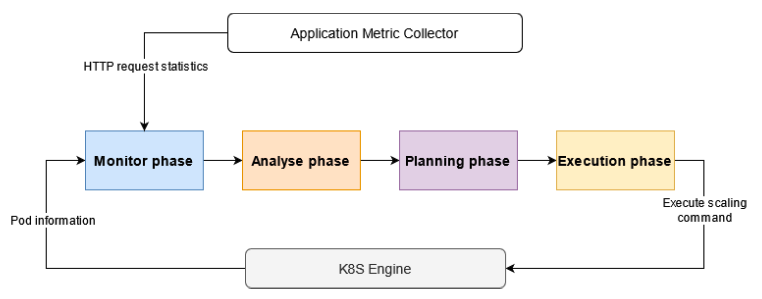
\includegraphics[width=0.8\textwidth]{chapter-2/mape.png}
    \caption{Arsitektur Sistem MAPE, \parencite{riset1}}
    \label{fig:mape}
\end{figure}

\subsection{Penelitian Lainnya}

Adapun \textit{autoscaler} yang sudah dikembangkan dan dibahas di banyak penelitian lain. Pendekatan dan metode yang digunakan sangat variatif. Gambaran umum mengenai penelitian lain yang berhubungan dengan \textit{autoscaler} menggunakan model prediksi, \textit{treshold} atau \textit{rule based} maupun \textit{machine learning} bisa dilihat pada tabel \ref{tab:overview-autoscaler}.

\begin{longtable}{|p{2in}|c|p{1in}|c|p{0.8in}|}

    \caption{Tabel Penelitian Lain terkait Pengembangan Metode \textit{Autoscaling}} \label{tab:overview-autoscaler} \\

    \hline
    \multicolumn{1}{|c|}{\textbf{Paper}} & \textbf{Virtualisasi} & \multicolumn{1}{|c|}{\textbf{Metrik}} & \textbf{Pendekatan} & \multicolumn{1}{|c|}{\textbf{Metode}} \\
    \hline
    \endfirsthead
    %
    \endhead
    %
    \textit{Intelligent Workload Factoring for a Hybrid Cloud Computing Model}, \parencite{zhang} & VM & \textit{Request Rate} & Reaktif & ARIMA \tabularnewline

    \textit{Autonomic Vertical Elasticity of Docker Containers with Elasticdocker}, \parencite{al2017autonomic} & \textit{Container} & Prosesor, Memori & Reaktif & \textit{Rule-based} \tabularnewline

    \textit{Horizontal Pod Autoscaler}, \parencite{hpa2} & \textit{Container} & Prosesor & Reaktif & \textit{Rule-based} \tabularnewline

    \textit{A Novel Resource Prediction and Provisioning Scheme in Cloud Data Center}, \parencite{rpps} & \textit{Container} & Prosesor & Proaktif & ARMA \tabularnewline

    \textit{Workload Prediction Using ARIMA Model and Its Impact on Cloud Applications QoS}, \parencite{workloadprediction} & VM & \textit{Request Rate} & Proaktif & ARIMA \tabularnewline

    \textit{Resource Elasticity Controller for Docker-based Web Applications}, \parencite{resourceelasticity} & \textit{Container} & \textit{Request Rate} & Proaktif & ARIMA \tabularnewline

    \textit{Combining Time Series Prediction Models using Genetic Algorithm to Autoscaling Web Applications Hosted in the Cloud Infrastructure}, \parencite{tspwithga} & - & \textit{Request Rate} & Proaktif & \textit{Genetic Algorithm} \tabularnewline

    \textit{Predicting Cloud Resource Provisioning using Machine Learning Techniques}, \parencite{predictcloudrsrc} & - & \textit{Task Length} & Proaktif & \textit{Artificial Neural Network} \tabularnewline

    \textit{Auto-scaling Microservices on IaaS under SLA with Cost-Effective Framework}, \parencite{asmicrocosteff} & VM & \textit{Request Rate} & Proaktif & \textit{Artificial Neural Network}, \textit{Recurrent Neural Network} \tabularnewline

    \textit{Machine Learning-based Auto-scaling for Containerized Applications}, \parencite{mlbasconapps} & \textit{Container} & \textit{Request Rate} & Proaktif & LSTM \tabularnewline

    \textit{Adaptive Horizontal Scaling of Microservices using Bi-LSTM}, \parencite{adaptivehsmicro} & \textit{Container} & Prosesor, Memori & Gabungan & Bi-LSTM \tabularnewline

    \hline
\end{longtable}

\section{\textit{Information Retrieval}}
\textit{Information Retrieval} (IR) adalah proses mencari bahan, biasanya berbentuk dokumen, yang bersifat tak terstruktur, biasanya teks, yang memenuhi kebutuhan informasi dari dalam koleksi besar \parencite{introtoinforetri}. IR saat ini sangat sering dilakukan contohnya dalam pencarian informasi berkaitan dengan representasi, penyimpanan, pengaturan, dokumen, halaman web, katalog online, catatan, dan objek multimedia. 

Tujuan utama dari IR adalah penyediaan akses yang efektif dan efisien ke informasi yang dibutuhkan oleh pengguna dalam situasi tertentu. Pengguna IR dapat beragam seperti individu, organisasi, maupun sistem yang membutuhkan informasi yang relevan. IR melibatkan penggunaan teknik-teknik seperti \textit{indexing, searching, retrieval,} dan \textit{evaluation} untuk memastikan informasi yang dihasilkan relevan, tepat, dan sesuai dengan kebutuhan pengguna.

Biasanya IR tersusun oleh beberapa komponen, diantaranya.
\begin{enumerate}
    \item \textit{Indexing}, proses mengubah dokumen menjadi bentuk yang lebih mudah dicari oleh sistem IR.
    \item \textit{Searching}, proses pencarian yang dilakukan oleh pengguna dengan memberikan \textit{query} ke dalam sistem IR dan sistem memberikan keluaran berupa dokumen yang paling relevan.
    \item \textit{Retrieval}, proses sistem IR mengambil dokumen yang relevan dan mengurutkan dokumen berdasarkan kesesuaian dengan \textit{query}.
    \item \textit{Evaluation}, proses penilaian kualitas sistem IR yang biasanya mencakup metrik evaluasi seperti \textit{precision}, \textit{recall}, dan skor F1. 
\end{enumerate}

Dalam melakukan proses-proses tersebut, komponen tersebut menggunakan beberapa teknik, diantaranya.
\begin{enumerate}
    \item \textit{Term Weighting}, teknik pemberian bobot terhadap kata-kata untuk membedakan yang lebih penting dan yang kurang.
    \item \textit{Query Expansion}, teknik menambahkan kata-kata yang relevan pada \textit{query} pengguna untuk meningkatkan akurasi hasil pencarian.
    \item \textit{Clustering}, teknik mengelompokkan dokumen yang mirip untuk memudahkan pengambilan.
\end{enumerate}

\section{Apache Lucene}
Apache Lucene adalah sebuah perpustakaan atau library open-source untuk Information Retrieval (IR) atau pencarian informasi yang berbasis teks. Lucene adalah \textit{library search engine} yang berkinerja tinggi dan berfitur lengkap. Lucene cocok untuk aplikasi yang memerlukan pencarian terstruktur, pencarian teks lengkap, pencarian pada graf dengan banyak node maupun vektor derajat tinggi, koreksi ejaan, atau saran kueri \parencite{apachelucene}. Lucene dikembangkan di bahasa pemrograman Java dan berfokus pada pencarian teks di dalam dokumen.

Lucene menggunakan model inverted index untuk mempercepat proses pencarian. Model ini mengubah dokumen yang diberikan menjadi indeks kata kunci atau \textit{term} dan menunjukkan letak setiap kata kunci tersebut muncul dalam dokumen. Indeks akan digunakan oleh Lucene untuk mencari kata kunci tertentu dalam dokumen dengan sangat cepat.

% \section{\textit{Inverted Index}}

\textit{Inverted Index} merupakan struktur data yang biasa digunakan untuk mesin pencari \parencite{invertedindex2}. Tujuan dari implementasi struktur data ini pada mesin pencari adalah untuk mengoptimalkan kecepatan query dalam mencari dokumen yang mengandung kata kunci tertentu. Struktur data ini melakukan pemetaan terhadap kata dan kumpulan tupel yang berisikan \textit{identifier} (ID) dokumen dan posisi karakter \parencite{invertedindex}. Struktur data ini biasanya dipakai untuk menggantikan \textit{Forward Index}. \textit{Forward Index} adalah struktur data yang menyimpan seluruh kata dalam sebuah dokumen sehingga jika \textit{forward index} di-\textit{query}, maka akan memerlukan iterasi sekuensial pada setiap dokumen dan kata kunci untuk membuktikan dokumen relevan. Sumber daya waktu, memori, dan pemrosesan yang dibutuhkan untuk melakukan query semacam itu tidak realistis dan praktis karena nyatanya, mesin pencari harus melakukan hal tersebut ke ratusan hinga jutaan dokumen. Dengan inverted index yang dibuat, query dapat diselesaikan dengan cara langsung melompat ke \textit{identifier} (ID) kata kunci melalui \textit{random access} pada inverted index untuk mendapatkan \textit{identifier} (ID) dokumen dan posisi karakter.

\section{\textit{Elastic Search}}
% \textit{Elastic Search} adalah aplikasi mesin pencarian RESTful.  \textit{Elastic Search} diciptakan sebagai pembungkus dan inovasi dari Apache Lucene yang sekedar hanya \textit{library} karena aplikasi yang beredar saat ini tidak hanya dibuat di atas Java dan membutuhkan fleksibilitas yang tinggi, sedangkan, Apache Lucene terkenal sangat sulit untuk orang awam yang tidak memahami istilah-istilah dan \textit{information retrieval}. \textit{Elastic Search} sendiri dibuat menggunakan Java namun menggunakan \textit{Application Programming Interface} RESTful melalui protokol HTTP sehingga aplikasi dengan bahasa apapun dapat dengan mudah menggunakan aplikasi ini. Tidak hanya itu, API dari \textit{Elastic Search} ini juga sudah sangat dipermudah sehingga pemakai tidak perlu mengetahui istilah-istilah dalam Apache Lucene. Sehingga, \textit{Elastic Search} ini sangat dekat dengan proses umum pada data seperti menyimpan, membaharui, menghapus, pengindeksan, pencarian, dan sebagainya.

\textit{Elastic Search} merupakan sebuah perangkat lunak \textit{open-source} yang ditulis menggunakan bahasa pemrograman Java. \textit{Elastic Search} dibangun di atas Apache Lucene. \textit{Elastic Search} menyimpan data secara terpusat untuk pencarian secepat kilat dan relevan \parencite{elasticsearchorigin}. Selain Apache Lucene, \textit{Elastic Search} memanfaatkan teknologi-teknologi lain untuk meningkatkan fungsionalitas dan performa, seperti Apache Hadoop untuk big data processing, Apache Spark untuk data analytics, dan Apache Storm untuk real-time stream processing.

\textit{Elastic Search} didesain sebagai sebuah sistem terdistribusi, yang berarti data yang disimpan pada \textit{Elastic Search} akan didistribusikan ke beberapa \textit{node} atau lebih dikenal sebagai \textit{sharding}, sehingga memungkinkan untuk meningkatkan performa, skalabilitas, dan ketahanan pada sistem. Sistem terdistribusi pada \textit{Elastic Search} dapat diatur dan dikonfigurasi agar dapat dijalankan pada beberapa \textit{node} yang terpisah atau pada \textit{cluster} yang terhubung, yang memungkinkan pengguna untuk menyimpan data yang sangat besar dan menjalankan query secara paralel pada beberapa node pada waktu yang bersamaan.

\textit{Elastic Search} dibuat untuk memudahkan pengguna mengakses data dan melakukan pencarian pada data yang besar dan kompleks dengan cepat dan efisien. Meskipun Apache Lucene telah menyediakan fitur-fitur yang bagus untuk \textit{indexing} dan \textit{searching}, tetapi Apache Lucene lebih fokus pada teknologi inti dan pengembangan secara \textit{information retrieval} seperti mengoptimisasi dan pengembangan \textit{indexing} dan \textit{searching}. Hal tersebut menyebabkan penggunaan Lucene memerlukan banyak pengaturan dan konfigurasi tambahan untuk bisa diintegrasikan dengan aplikasi yang lebih besar. Dalam hal ini, \textit{Elastic Search} hadir sebagai sebuah solusi yang lebih terintegrasi, mudah digunakan, dan dapat diatur secara fleksibel. \textit{Elastic Search} memanfaatkan Lucene sebagai mesin pencari, tetapi menambahkan banyak fitur-fitur dan fungsionalitas tambahan untuk meningkatkan performa dan kemudahan penggunaan. Selain itu, \textit{Elastic Search} dirancang sebagai aplikasi dengan sistem terdistribusi dan \textit{scalable} yang memungkinkan data terdistribusi di beberapa node atau \textit{sharding}, sehingga memungkinkan \textit{Elastic Search} untuk mengatasi masalah data yang sangat besar dan kompleks secara efektif dan efisien. Sedangkan, Lucene hanya pada batas kakas atau \textit{library}.

\textit{Elastic Search} dapat digunakan dengan protokol HTTP dan REST API. Dalam penggunaan dengan protokol HTTP, \textit{Elastic Search} menyediakan endpoint API RESTful HTTP yang dapat diakses oleh pengguna dengan memakai klien HTTP, seperti perintah cURL, \textit{Postman} atau \textit{web browser}. Pengguna dapat membuat permintaan HTTP seperti GET, POST, PUT, DELETE ke API endpoint melalui klien HTTP, dan \textit{Elastic Search} akan memberikan respon sesuai dengan permintaan.

Dalam \textit{Elastic Search} terdapat beberapa operasi yang dapat dilakukan, diantaranya:
\begin{enumerate}
    \item \textit{Index}
    
    Operasi ini akan dijelaskan secara khusus pada bagian selanjutnya, \ref{sec:index}.

    \item \textit{Get}
    
    Operasi \textit{Get} digunakan untuk mengambil dokumen individual berdasarkan ID-nya dari indeks tertentu.
    
    \item \textit{Query}
    
    \textit{Query} digunakan untuk melakukan pencarian dan pengambilan data yang sesuai dengan kriteria tertentu. \textit{Elasticsearch} menyediakan berbagai jenis query seperti pencarian teks lengkap, pencocokan kata kunci, pencocokan frasa, pencarian fuzzy, dan lain-lain.
    
    \item \textit{Fetch}
    
    \textit{Fetch} adalah proses pengambilan dokumen lengkap dari indeks setelah melakukan query. Saat ditemukan, \textit{Elasticsearch} mengambil dokumen dari indeks dan akan digunakan sebagai respon kepada pengguna.
    
    \item \textit{Scroll}
    
    \textit{Scroll} adalah mekanisme pengambilan dokumen yang banyak dari hasil pencarian tanpa perlu mengirimkan \textit{query} ulang. Hal ini menyebabkan pengambilan dokumen dapat menjadi lebih efisien dalam beberapa permintaan, namun, dalam beberapa kasus, bisa menjadi lebih lama untuk mengambil semua dokumen yang relevan.
    
    \item \textit{Suggest}
    
    \textit{Suggest} adalah mekanisme untuk memberikan saran atau \textit{autocompletion} saat pengguna memasukkan kata kunci atau frasa. Biasanya digunakan untuk \textit{autocompletion}, pengoreksi kesalahan pengejaan, dan saran pencarian lainnya.
    
    \item \textit{Bulk}
    
    \textit{Bulk} adalah operasi yang digunakan untuk memasukkan atau memperbarui beberapa dokumen dalam satu permintaan.
    
    \item \textit{Flush}
    
    \textit{Flush} adalah operasi yang digunakan untuk mengosongkan memori \textit{cache} dan menulis data yang tertunda ke disk. Operasi ini memastikan bahwa data yang ditulis telah disimpan secara permanen di indeks.
    
    \item \textit{Refresh}
    
    \textit{Refresh} adalah operasi yang digunakan untuk membuat perubahan yang terjadi pada indeks secara terlihat dan dapat dicari. Saat melakukan operasi indeks seperti menambahkan atau menghapus dokumen, perubahan tersebut tidak langsung terlihat oleh pencarian hingga dilakukan operasi refresh.
\end{enumerate}

\section{Java \textit{Virtual Machine}}
\textit{Java Virtual Machine} atau JVM adalah program yang dapat membaca program java yang telah dikompilasi atau biasa dikenal sebagai \textit{java bytecode} dan menginterpretasikannya menjadi bahasa mesin yang dapat dieksekusi oleh komputer \parencite{java12}. Secara tidak langsung, JVM merupakan komponen utama dalam menjalankan program bahasa Java. Struktur JVM terdiri dari \textit{runtime data structure} di memori dan dua subsistem yang berhubungan langsung dengan \textit{runtime data structure} yaitu \textit{class loader} dan \textit{execution engine}. Semua program yang dibuat dengan Java akan dikompilasi ke \textit{java bytecode} yang nantinya akan diinterpretasikan oleh JVM untuk dieksekusi komputer.

\textit{Elastic Search}, yang terbuat dari bahasa Java, berjalan di atas platform Java Virtual Machine (JVM). JVM sendiri akan bertanggung jawab untuk menjalankan kode Java dan mengelola sumber daya yang dibutuhkan oleh program, seperti memori, prosesor, dan jaringan. Sehingga, JVM memiliki peran penting dalam menjalankan \textit{Elastic Search} dan memastikan performanya baik. JVM menyediakan opsi pengaturan yang membuat pengguna dapat mengontrol alokasi memori dan penggunaan CPU pada aplikasi \textit{Elastic Search}. Dengan mengatur parameter JVM yang tepat, pengguna dapat memperbaiki kinerja \textit{Elastic Search} dan memaksimalkan penggunaan sumber daya sistem.

Parameter yang berhubungan erat dengan alokasi sumber daya pada \textit{Elastic Search} dan mempengaruhi kinerja JVM adalah parameter \textit{heap size} (-Xms dan -Xmx) yang mengatur ukuran \textit{heap memory} yang dialokasikan untuk JVM. \textit{Heap memory} adalah tempat JVM menyimpan objek dan data dari aplikasi Java yang sedang berjalan. Parameter -Xms menentukan ukuran \textit{heap memory} awal yang dialokasikan ketika JVM dimulai, sedangkan parameter -Xmx menentukan batas maksimal ukuran \textit{heap memory} yang dapat dipakai oleh JVM. Selain itu, terdapat parameter lain yang dapat mempengaruhi kinerja JVM dan \textit{Elastic Search}, seperti \textit{thread pool size}, \textit{circuit breaker settings}, dan lain-lain. Parameter-parameter ini dapat diatur melalui file konfigurasi \textit{Elastic Search} atau melalui command line arguments saat menjalankan \textit{Elastic Search}.

% \section{\textit{Indexing}}
\label{sec:index}

\textit{Indexing} adalah suatu teknik untuk menyusun kata-kata dan mengurangi usaha untuk mencari hal yang berkaitan dengan kata tersebut jika diperlukan, \parencite{database}. Secara umum, indeks banyak digunakan pada buku teks, basis data, dan sistem information retrieval. Seperti salah satu contoh tekniknya adalah \textit{Inverted Index} yang telah dijelaskan pada \ref{sec:invertedindex}.

Terdapat kelebihan penggunaan indeks, diantaranya:
\begin{enumerate}
    \item \textit{Indexing} dapat mempercepat proses pencarian data dengan membuat indeks dan mencocokkan kata kunci dengan indeks tersebut, sehingga mesin dapat menemukan data dengan lebih cepat.
    \item \textit{Indexing} dapat meningkatkan akurasi pencarian dengan menampilkan hasil pencarian yang lebih relevan dengan kata kunci yang dimasukkan.
\end{enumerate}

Namun, ada juga kelemahan dari penggunaan indeks, yaitu sebagai berikut.
\begin{enumerate}
    \item \textit{Indexing} memerlukan ruang penyimpanan tambahan untuk membuat indeks.
    \item Proses pembuatan \textit{indexing} memerlukan waktu, terutama jika data yang akan di-indeks sangat banyak.
\end{enumerate}

Sehingga, dapat disimpulkan penggunaan indeks sangat bermanfaat namun menambahkan biaya.
Pada kasus-kasus dokumen besar, penggunaan indeks pengaruhnya sangat besar karena mesin akan mencari data pada indeks terlebih dahulu sebelum mencari data pada dokumen asli. Hal ini dapat membantu mengurangi waktu pencarian dan menghemat penggunaan memori karena mesin tidak perlu membaca seluruh dokumen untuk menemukan data yang dicari. Namun, apabila \textit{indexing} dilakukan secara berlebihan, akan terdapat banyak indeks yang tidak terpakai dan hanya akan menambah kebutuhan memori.

% Konsep \textit{caching} sendiri adalah menyimpan data yang sering diakses pada level cache atau memori yang lebih dekat dengan CPU agar dapat diakses dengan cepat saat ingin melakukan pencarian, lihat gambar \ref{fig:cache-level}. \textit{Cache} sendiri biasanya memiliki ruang yang terbatas sehingga biasanya membuang data yang sudah tidak diakses sehingga jika dibutuhkan harus dicari ke \textit{storage}. Konsep ini ditiru oleh basis data dan aplikasi \textit{information retrieval} untuk mempercepat proses pencarian dengan memanfaatkan \textit{indexing} untuk mencari (lihat gambar \ref{fig:cache-app}) dan \textit{caching} untuk mengembalikan data yang sering diakses dengan memanfaatkan memori.

% \begin{figure}[h]
%     \centering
%     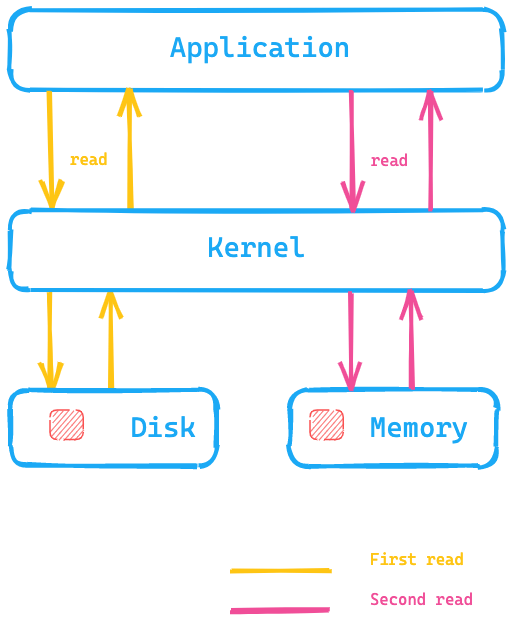
\includegraphics[width=0.5\textwidth]{chapter-2/cache-app.png}
%     \caption{Prinsip Cache pada Aplikasi}
%     \label{fig:cache-app}
% \end{figure}

% \begin{figure}[h]
%     \centering
%     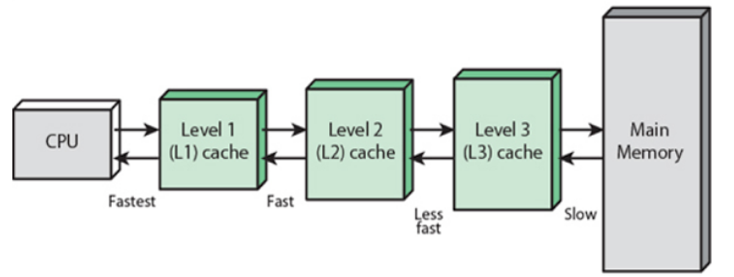
\includegraphics[width=0.5\textwidth]{chapter-2/cache-memory.jpeg}
%     \caption{Level-level pada Cache}
%     \label{fig:cache-level}
% \end{figure}

% \section{\textit{Caching}}

% \section{Simulasi dengan \textit{Elastic Search Benchmarking}}

\textit{Elastic Search Benchmarking} adalah metode yang digunakan untuk melakukan simulasi beban pada \textit{Elastic Search}. Dengan menggunakan \textit{Elastic Search Benchmarking}, pengguna dapat memprediksi jumlah beban yang dapat ditangani oleh \textit{Elastic Search} dan melakukan pencarian terhadap \textit{bottleneck} untuk diperbaiki.

\textit{Elastic Search Benchmarking} memiliki banyak cara pengujian seperti uji beban, uji rentang kisaran, uji keseimbangan, dan uji kestabilan. Uji beban bertujuan untuk mengukur jumlah beban yang dapat ditangani pada suatu waktu tertentu. Uji rentang kisaran dapat digunakan untuk membandingkan kinerja dari setiap rentang data pada variasi yang ada. Uji keseimbangan bertujuan untuk membandingkan kinerja sistem yang memiliki banyak \textit{node} pada sebuah \textit{cluster}. Terakhir, uji kestabilan digunakan untuk menguji kinerja sistem dalam penggunaan waktu yang lama.

\textit{Elastic Search Benchmarking} dapat digunakan untuk memprediksi besar biaya yang diperlukan untuk menjalankan \textit{Elastic Search} pada tingkat beban tertentu. Tak hanya itu, \textit{Elastic Search Benchmarking} dapat digunakan untuk mengidentifikasi titik lemah dan memberikan informasi yang berguna untuk meningkatkan kinerja sistem.

Salah satu tools untuk melakukan \textit{Elastic Search Benchmarking} adalah Rally. Tools ini dapat digunakan untuk mengukur kinerja \textit{Elastic Search} dalam berbagai situasi, termasuk pada lingkungan yang kompleks dan besar. Selain itu, Rally juga menyediakan sejumlah besar skenario pengujian kinerja bawaan yang dapat digunakan untuk menguji kinerja \textit{Elastic Search} dengan berbagai konfigurasi dan skenario pengujian yang berbeda. 
% \section{Pembelajaran Mesin}
% Pembelajaran Mesin adalah sebuah bidang pembelajaran yang mempelajari pemahaman dan membangun metode untuk "belajar" dengan memanfaatkan data untuk meningkatkan banyak aspek terutama efisiensi dan kualitas terhadap suatu rangkaian tugas. Algoritma pembelajaran mesin membangun model berdasarkan data sampel yang biasa disebut \textit{training data} untuk menghasilkan model yang dapat memprediksi atau membuat keputusan tanpa diprogram secara eksplisit, \parencite{ml}.

% \subsection{\textit{Reinforcement Learning}}
% \textit{Reinforcement learning} atau RL adalah bidang pembelajaran mesin yang mengotomasi sebuah agen untuk mengambil tindakan dan memaksimalkan \textit{reward} dari aksi yang dilakukan, \parencite{reinforcementlearning}. RL adalah salah satu paradigma dari tiga pembelajaran mesin dasar seperti \textit{Supervised Learning} dan \textit{Unsupervised Learning}. Singkatnya, RL membuat agen dapat mengoreksi pengetahuannya secara terus menerus agar dapat memaksimalkan fungsinya. Berbeda dengan \textit{Supervised Learning}, RL tidak memerlukan label dan tidak memerlukan secara eksplisit dikoreksi. Fokus dalam membangun RL, adalah mencari keseimbangan eksplorasi terhadap lingkungan baru dan eksploitasi terhadap pengetahuan yang dimiliki.

% penelitian terkait
% \blankpage
\chapter{Analisis Persoalan dan Rancangan Solusi}

Tujuan utama penulisan bab ini adalah untuk menguraikan rencana penyelesaian masalah tugas akhir yang akan dieksekusi secara utuh pada saat pelaksanaan Tugas Akhir II. Bab ini merupakan bab penutup Laporan Tugas Akhir I yang dapat dipandang sebagai bab yang akan menjembatani perpindahan ke proses pelaksanaan Tugas Akhir II. Pengembangan lebih lanjut dari bab ini dapat menjadi bagian dari bab Deskripsi Solusi pada Laporan Tugas Akhir.

\section{Analisis Persoalan}

Basis data, \textit{information retrieval} dan server memori seringkali digunakan sebagai \textit{technology stack} aplikasi zaman sekarang.
Ketiga jenis aplikasi ini akan menggunakan memori semaksimal yang mereka dapat gunakan ketika memiliki jumlah data yang besar.
Kegunaan dari memakai memori biasanya dipakai untuk melakukan \textit{caching} yang sebenarnya pada aplikasi skala besar tidak akan terlalu signifikan karena permintaan masuk yang terlalu beragam. 
Akibatnya, memori yang ditahan oleh aplikasi tersebut tidak dapat digunakan oleh aplikasi lainnya.
Permasalahan ini lebih nyata terasa ketika aplikasi tersebut diletakkan pada sebuah \textit{pods} Kubernetes. Karena, sebuah \textit{pods} harus bisa dimuat dalam sebuah \textit{node} yang sumber dayanya terbatas dan belum tentu berukuran besar. Meskipun \textit{cloud} seringkali dianggap sumber daya tak terbatas, namun penggunaan memori yang terlalu besar dan tidak berakibat terlalu signifikan terhadap performa adalah sangat tidak efisien.

Salah satu aplikasi \textit{information retrieval} yang sering dipakai adalah \textit{Elastic Search}. 
Aplikasi ini membungkus kakas \textit{Apache Lucene} yang dipermudah dengan membuat standar antarmuka berupa \textit{HTTP Request}.
\textit{Elastic Search} juga diciptakan guna untuk menghilangkan keterbatasan bahasa, hanya aplikasi berbasis Java yang dapat menggunakan kakas \textit{Apache Lucene}.
Sayangnya, aplikasi ini sangat boros dalam hal memori dan cenderung untuk mengambil memori sebanyak yang diberikan.

\textit{Elastic Search} dijalankan diatas \textit{Java Virtual Machine} (JVM) yang pada umumnya memiliki command flag untuk membatasi memori yang akan digunakan. Tidak hanya itu, \textit{Kubernetes Pods} juga memiliki parameter berupa \textit{resource limit} yang dapat diubah-ubah untuk membatasi penggunaan CPU dan memori. Cara tersebut dapat dilakukan jika ingin diraih efisiensi sumber daya dengan mengacuhkan kinerja dari aplikasi dan kondisi jumlah permintaan dalam satu satuan waktu dalam jangka waktu tertentu. Oleh karena itu, diperlukan kontrol adaptif yang mengubah secara dinamis.

\section{Analisis Solusi}

Untuk membuat kontrol adaptif untuk menangani masalah efisiensi sumber daya berdasarkan kinerja aplikasi serta kondisi jumlah permintaan dalam satu satuan waktu dalam jangka waktu tertentu, akan diajukan dua buah pendekatan solusi. Berikut adalah analisis dari dua pendekatan yang diajukan pada tugas akhir ini.

\subsection{Vertical Pod Autoscaler dari Kubernetes}

Kubernetes sendiri saat ini sedang mengembangkan Vertical Pod Autoscaler (VPA), \parencite{vpa}. Fitur ini sudah bisa dipakai meskipun masih dalam tahap pengembangan. Namun, jika menggunakan pendekatan ini, terdapat beberapa \textit{drawback}. Pertama, VPA perlu melakukan \textit{restart} terhadap \textit{pod} yang ingin dibesarkan sedangkan \textit{Elastic Search} menggunakan sistem sharding, apabila mematikan salah satu \textit{Node Elastic Search} maka hal tersebut akan menyebabkan \textit{Elastic Search} perlu melakukan \textit{balancing shard data} setiap kali \textit{autoscale} yang tentunya akan memakan ketersediaan dan sumber daya. Kedua, VPA menggunakan \textit{metrics} yang didapatkan dari Kubernetes bukan dari Elastic Search, hal ini akan menyebabkan kurangnya akurasi dan atau tidak tercapainya tujuan untuk membebaskan memori yang dipakai namun dampaknya tidak signifikan terhadap kinerja \textit{Elastic Search} itu sendiri. Oleh karena itu, rancangan solusi dengan hal ini dirasa kurang cocok.

\subsection{Sistem Kontrol Adaptif}
\label{sec:sistemkontroladaptif}

Sistem Kontrol Adaptif akan memanfaatkan \textit{metrics} yang didapat dari \textit{Elastic Search} secara periodik. Data tersebut akan dijadikan faktor dalam membuat keputusan untuk memperbesar atau memperkecil limit memori \textit{Elastic Search} tersebut. Sistem tersebut secara umum akan dibagi menjadi dua komponen, yaitu \textit{Metrics Collector} dan \textit{Memory Controller}.

\section{Rancangan Solusi}

Seperti yang sudah dijelaskan pada bagian sebelumnya, \ref{sec:sistemkontroladaptif}, Sistem Kontrol Adaptif akan disusun atas dua komponen, yaitu sebagai berikut.
\subsection{Komponen \textit{Metrics Controller}}
\label{sec:metricscontroller}

Komponen ini bertugas untuk menarik data \textit{metrics} dari \textit{Elastic Search} menggunakan HTTP Client dan Database Connector Client. Data tersebut lalu akan disimpan ke sebuah database relasional yang dapat digunakan sebagai data historis. Sehingga, kedepannya dapat dilakukan analisis diagnostik dan analisis prediktif.

\subsection{Komponen \textit{Memory Controller}}

Komponen ini bertugas untuk membuat keputusan untuk memperbesar, membiarkan atau memperkecil limit memory \textit{Elastic Search}. Komponen ini akan menggunakan data yang dikumpulkan oleh komponen Metrics Controller, \ref{sec:metricscontroller}. Kakas yang akan digunakan oleh komponen ini adalah Kubernetes Client Library, Database Connector Client, dan Library Machine Learning, jika diperlukan.

Adapun algoritma yang akan digunakan untuk membuat keputusan. Saat ini ada beberapa pilihan algoritma yang dapat diterapkan sebagai pembuat keputusan.

\subsubsection{Greedy, Trial and Error}
\label{sec:greedytrialerror}

Secara periodik, algoritma ini akan memaksa memangkas limit memori sebesar 50 persen dari kondisi sekarang.
Apabila kinerja \textit{Elastic Search} memburuk, algoritma akan mengembalikan limit memori sebesar 50 persen dari kondisi saat itu.
Hal ini akan terus dilakukan sampai konfigurasi algoritma sistem diubah.

\subsubsection{Linear Support Vector Machine}

Awalnya, algoritma ini akan memakai algoritma sebelumnya, \ref{sec:greedytrialerror}, untuk mengumpulkan data.
Setelah data terkumpul, algoritma ini akan memprediksi menggunakan Linear Support Vector Machine untuk memutuskan melakukan peningkatan atau pengurangan limit memori.
Jika terjadi perubahan trend, algoritma akan melakukan training ulang dari data-data terbaru.
Linear Support Vector Machine ini akan menerima \textit{input} berupa memori yang dipakai, \textit{request per second}, waktu untuk melakukan pencarian, waktu untuk melakukan aggregasi, waktu untuk melakukan penggabungan.
\chapter{Implementasi dan Pengujian}
Bab ini akan menjelaskan proses implementasi dari rancangan solusi yang telah dikaji pada Bab III. Setelah pembahasan terkait implementasi, akan dilanjutkan dengan pemaparan hasil uji terkait implementasi yang telah dibuat.

\section{Lingkungan}

\textit{Autoscaler} berbasis kontrol fleksibel akan diimplementasikan di lingkungan komputer lokal. Berikut adalah lingkungan perangkat keras dan perangkat lunak secara terperinci.

Implementasi sistem tugas akhir dilakukan dengan mengimplementasikan dengan bantuan beberapa kakas pada bahasa \textit{python}. Sistem akan hidup di luar \textit{kubernetes cluster} dan mengakses Kubernetes beserta \textit{pods}-nya melalui \textit{Kubernetes Client Library} dan \textit{service Elastic search} melalui \textit{web service} yang dapat diakses dari luar \textit{cluster}.

\textit{Autoscaler} berbasis kontrol fleksibel akan berjalan di \textit{cluster} Kubernetes lokal. Adapun spesifikasi dari komputer yang dipakai untuk pengembangan adalah sebagai berikut.
\begin{enumerate}
    \item \textbf{Perangkat Keras}
    
        \begin{enumerate}
            \item CPU: \textit{Apple M1 Chip}
            \item RAM: 16 GB
        \end{enumerate}
    
    \item \textbf{Perangkat Lunak}
        
        \begin{enumerate}
            \item Platform dan Sistem Operasi: Darwin AMD64, MacOS Monterey 12.6
            \item \textit{Containerization}: Docker
            \item \textit{Kubernetes Cluster}:
                \begin{enumerate}
                    \item Kubernetes Client v1.27.1-eks-2f008fe
                    \item Kubernetes Docker Desktop: Kubernetes v1.25.9
                \end{enumerate}
            \item Bahasa: Python 3.9.12
            \item Dependensi Lain:
                \begin{enumerate}
                    \item \textit{Kubernetes Client Library}
                    \item \textit{Pandas, numpy, statsmodels dan pmdarima}
                    \item \textit{Pickle}
                \end{enumerate}
        \end{enumerate}
\end{enumerate}

\section{Implementasi}

Bagian ini akan menjelaskan tentang implementasi sistem kontrol adaptif secara terperinci.

\subsection{Batasan Implementasi}
Berikut adalah batasan yang ditetapkan dalam melakukan implementasi sistem kontrol adaptif.
\begin{enumerate}
    \item Masih menerapkan sistem \textit{single node} dan \textit{single pod}.
    \item Tidak memperhatikan optimalisasi dari model ARIMA.
    \item Hanya dapat menangani \textit{metrics} yang sudah ditentukan, yaitu \textit{throughput} dari setiap operasi \textit{Elastic Search} serta utilisasi prosesor hingga memori.
    \item Tidak mempertimbangkan besarnya model seiring bertambahnya data.
    \item Komponen \textit{Metrics Fetcher} berjalan di proses lain dan diimplementasikan dalam \textit{script} yang berbeda dikarenakan bahasa Python memiliki kekurangan dalam penanganan \textit{multithreading}.
    \item Pertukaran data antara komponen \textit{Metrics Fetcher} dan \textit{Predictor} melalui stream file.
\end{enumerate}

\subsection{Kakas yang Digunakan}
Dalam melakukan implementasi ini diperlukan beberapa kakas, diantaranya adalah sebagai berikut.
\begin{enumerate}
    \item \textit{Docker}, \textit{Docker Desktop} dan \textit{Docker Desktop Kubernetes} untuk dipakai sebagai \textit{containerization} dan \textit{cluster} kubernetes lokal.
    \item Minikube dipakai sebagai \textit{cluster} kubernetes lokal dengan versi yang lebih baru karena versi \textit{Docker Desktop Kubernetes} hanya memakai yang \textit{stable} dan tidak bisa dipaksa naik versi.
    \item Pandas dan Numpy untuk keperluan \textit{data processing} serta bentuk data untuk dikirimkan ke komponen lain serta model prediksi ARIMA.
    \item \textit{Kubernetes Python Client} untuk mengontrol \textit{cluster} kubernetes melalui kode Python.
    \item \textit{Pickle} untuk menyimpan model ARIMA sehingga persisten meskipun sistem di-\textit{restart}.
    \item \textit{Statsmodels} dan \textit{pmdarima} untuk membangun model ARIMA serta melakukan otomasi pencarian orde atau lebih dikenal sebagai Auto-ARIMA.
\end{enumerate}

% TODO Untuk spesifikasi pods 

\subsection{Sistem Kontrol Adaptif dengan Model Prediktif berbasis \textit{Time Series}}

Seperti yang sudah dijelaskan pada bagian rancangan solusi (\ref{sec:rancangan-solusi}), sistem kontrol adaptif akan diimplementasikan dengan beberapa komponen penyusun, diantaranya adalah sebagai berikut.

% TODO \subsubsection{Tampilan Implementasi}

\subsection{Eksperimen \textit{In-place Resource Resize} untuk \textit{pods Kubernetes}}

Pada bagian sebelumnya, diperlukan \textit{resizing} sumber daya yang dialokasikan untuk \textit{pods} yang sedang berjalan tanpa melakukan \textit{restart}. Untuk hal tersebut, perlu dilakukan eksperimen, berikut adalah rincian dari eksperimen yang telah dilakukan.

\subsubsection{Pendahuluan}

\textit{In-place Resource Resize} adalah fitur untuk mengubah ukuran sumber daya CPU dan memori yang dialokasikan untuk kontainer pada pod yang sedang berjalan tanpa harus me-\textit{restart} pod atau kontainernya. Sebuah \textit{node} Kubernetes mengalokasikan sumber daya untuk sebuah pod berdasarkan permintaannya, dan membatasi penggunaan sumber daya pod berdasarkan batasan yang ditentukan dalam kontainer-kontainer pod tersebut. Fitur ini baru hadir pada versi Kubernetes 1.27.0, dan, pada saat tugas akhir ini dikerjakan, masih dalam tahap \textit{alpha testing} dan pengembangan. Berdasarkan \parencite{kubeinplaceupdate2}, dokumentasi resmi dipublikasikan pada 30 Maret 2023 7:59 PM PST. Sedangkan berdasarkan \parencite{kubeinplaceupdate}, publikasi \textit{alpha testing} semenjak 13 Mei 2023.

\subsubsection{Pengerjaan Eksperimen}
Dalam melakukan eksperimen ini, dilakukan beberapa tahap sebagai berikut.

\begin{enumerate}
    \item Memastikan versi Kubernetes yang digunakan adalah versi 1.27.0 atau lebih baru pada \textit{client} dan \textit{server}.
    
    Pada saat itu, Kubernetes lokal yang dipakai adalah \textit{Docker Desktop Kubernetes} yang membatasi versi Kubernetes pada versi 1.25.9. Sehingga, dilakukan pengubahan server dengan menggunakan Minikube. Sayangnya, versi maksimal yang bisa dipakai oleh Minikube adalah Kubernetes versi 1.27.0-rc0, versi 1.27 yang paling pertama atau \textit{release candidate 0}. Untuk mengecek bisa dilihat pada \url{https://github.com/kubernetes/minikube/releases/tag/v1.30.0}. Dicoba juga untuk dipaksa menggunakan versi 1.27.1 maupun 1.27.3, namun hal tersebut gagal untuk dilakukan. Sehingga, untuk eksperimen ini, digunakan Kubernetes versi 1.27.0-rc0 melalui Minikube.

    \item Membuat \textit{deployment} yang akan digunakan untuk eksperimen.
    
    Konfigurasi \textit{deployment} berubah, karena untuk menggunakan fitur ini, tidak bisa membuat \textit{pods} dengan menggunakan tipe \textit{deployment} melainkan harus langsung membuat dengan tipe \textit{pod}. Terdapat juga beberapa konfigurasi baru yang perlu diatur.

    \item Mengeksekusi perintah untuk melakukan \textit{in-place resource resize}.
    
    Hal ini bisa dilakukan dengan mengeksekusi perintah \textit{patch pod}. Perintah ini bisa dilihat pada dokumentasi: \url{https://kubernetes.io/docs/tasks/configure-pod-container/resize-container-resources/}.

    Saat hal ini dijalankan terdapat pesan eror yang mengatakan bahwa fitur \textit{patch} tersebut hanya bisa dilakukan selain resource. Padahal, inisiasi eksperimen sudah disesuaikan dengan \textit{requirement} yang disebutkan pada dokumentasi.

    \item Mengecek detail informasi \textit{pods}
    
    Seharusnya, ketika mengecek detail informasi \textit{pods} akan terlihat bahwa resource yang digunakan sudah berubah dan terdapat informasi-informasi baru yang hanya muncul pada versi terbaru Kubernetes. Namun, hal ini tidak terjadi. Resource yang digunakan masih sama dengan sebelumnya. Dan hasil detail informasi sebuah \textit{pods} tidak memperlihatkan detail informasi terbaru yang sesuai dengan contoh pada dokumentasi.
\end{enumerate}

\subsubsection{Hasil Eksperimen}

Berdasarkan hasil eksperimen tersebut, dapat disimpulkan bahwa.

\begin{enumerate}
    \item Fitur \textit{in-place resource resize} belum bisa digunakan pada Kubernetes versi 1.27.0-rc0.
    \item Melakukan \textit{resource resize} tanpa melakukan \textit{restart} mungkin bisa dilakukan pada masa yang akan datang.
    \item Eksperimen ini bisa dicoba lagi pada masa yang akan datang. Mengingat tools kubernetes lokal masih belum bisa menggunakan versi \textit{alpha} terbaru. Dan, pada saat ini, fitur ini masih dalam tahap \textit{alpha testing} dan pengembangan.
\end{enumerate}

Sehingga, untuk saat ini, eksperimen ini tidak bisa dilakukan lebih jauh lagi. Dan oleh karena itu, sistem kontrol adaptif yang dibuat masih memakai sistem \textit{Rolling Update} untuk mengubah sumber daya alokasi. Namun, kedepannya, jika ingin diteruskan, besar kemungkinan hal ini bisa dilakukan karena dari Kubernetes sendiri sedang mengembangkan fitur tersebut.

\section{Pengujian}

Bagian ini akan menjelaskan beberapa skenario yang dilakukan untuk menguji sistem kontrol adaptif. Pengujian akan dilakukan per komponen lalu dilanjutkan dengan satu sistem penuh. Setiap skenario pengujian akan dijelaskan tujuannya, skenario yang dilakukan, dan hasil pengujian yang didapatkan.

% \subsection{Pengujian X}

% \subsubsection{Tujuan Pengujian}

% \subsubsection{Skenario Pengujian}

% \subsubsection{Hasil Pengujian dan Analisis}

\subsection{Pengujian Komponen \textit{Metrics Fetcher}}

Pada bagian ini akan dijelaskan tentang tujuan, skenario, hasil, dan analisis dari pengujian komponen \textbf{\textit{Metrics Fetcher}}.

\subsubsection{Tujuan Pengujian}

Tujuan pengujian ini memastikan komponen \textbf{\textit{Metrics Fetcher}} dapat berjalan dengan baik dan menghasilkan data yang sesuai dengan ekspektasi.

\subsubsection{Skenario Pengujian}

Pengujian terhadap komponen \textbf{\textit{Metrics Fetcher}} dilakukan dengan beberapa skenario sebagai berikut serta ekspektasi dari pengujian yang dilakukan.
\begin{enumerate}
    \item \textit{Elastic Search} sedang \textit{idle}.
        Data yang diminta dari \textit{Node Stats API} diekspektasikan relatif statis dan berhasil diletakkan pada \textit{stream file}.
    \item \textit{Elastic Search} sedang digunakan untuk melakukan operasi penambahan data.
        Data yang diminta dari \textit{Node Stats API} seharusnya relatif berubah terutama pada aspek \textit{throughput} operasi \textit{index} dan \textit{bulk}. Lalu, data tersebut diekspektasikan berhasil diletakkan pada \textit{stream file}.
    \item \textit{Elastic Search} sedang digunakan untuk melakukan operasi pencarian data.
        Data yang diminta dari \textit{Node Stats API} seharusnya relatif berubah terutama pada aspek \textit{throughput} operasi \textit{query} dan \textit{fetch}. Lalu, data tersebut diekspektasikan berhasil diletakkan pada \textit{stream file}.
\end{enumerate}

\subsubsection{Hasil Pengujian dan Analisis}

Hasil untuk skenario 1 dapat dilihat pada gambar \ref{fig:mf-1}. Data yang ditarik sudah relatif statis untuk semua aspek dan berhasil diletakkan pada \textit{stream file}. Untuk skenario 2, dapat dilihat pada gambar \ref{fig:mf-2}. Data yang ditarik sudah mengalami perubahan pada operasi \textit{index} dan \textit{bulk} serta berhasil diletakkan pada \textit{stream file}. Terakhir, skenario 3, dapat dilihat pada gambar \ref{fig:mf-3}. Data yang ditarik sudah mengalami perubahan pada operasi \textit{query} dan \textit{fetch} serta berhasil diletakkan pada \textit{stream file}.

\begin{figure}[h]
    \centering
    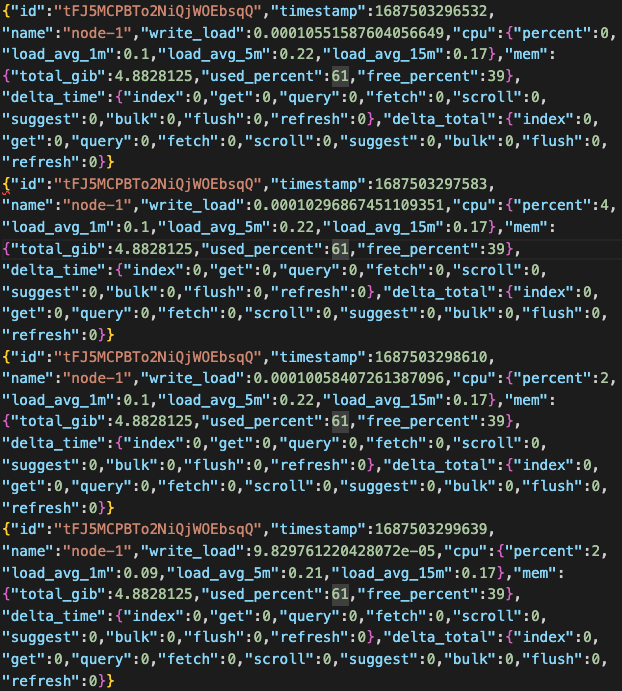
\includegraphics[width=0.8\textwidth]{chapter-4/mf-1.png}
    \caption{Hasil Pengujian Komponen \textit{Metrics Fetcher} Skenario 1}
    \label{fig:mf-1}
\end{figure}

\begin{figure}[h]
    \centering
    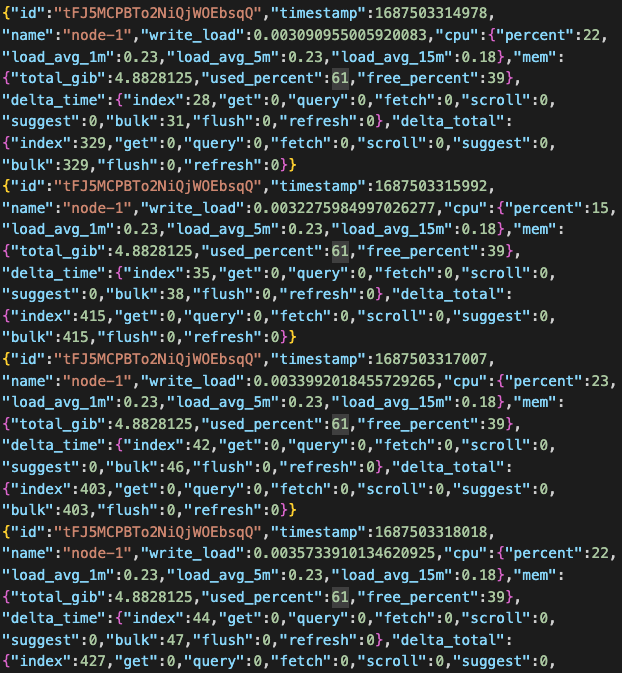
\includegraphics[width=0.8\textwidth]{chapter-4/mf-2.png}
    \caption{Hasil Pengujian Komponen \textit{Metrics Fetcher} Skenario 2}
    \label{fig:mf-2}
\end{figure}

\begin{figure}[h]
    \centering
    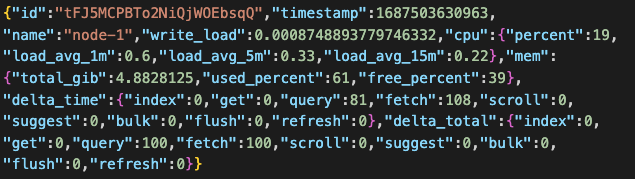
\includegraphics[width=0.8\textwidth]{chapter-4/mf-3.png}
    \caption{Hasil Pengujian Komponen \textit{Metrics Fetcher} Skenario 3}
    \label{fig:mf-3}
\end{figure}

Maka untuk pengujian komponen \textbf{\textit{Metrics Fetcher}} sudah sesuai ekspektasi dan dapat dilanjutkan ke pengujian komponen lainnya.
\subsection{Pengujian Komponen \textit{Rule Manager}}
\subsection{Pengujian Komponen \textit{Predictor}}
\subsection{Pengujian Komponen \textit{Resource Controller}}
\subsection{Pengujian Sistem \textit{Adaptive Control}}

Pada bagian ini akan dijelaskan tentang tujuan, skenario, hasil, dan analisis dari pengujian sistem sekaligus komponen \textbf{\textit{Adaptive Control}}.

\subsubsection{Tujuan Pengujian}

Tujuan pengujian ini memastikan sistem \textbf{\textit{Metrics Fetcher}} dapat berjalan dengan baik dan menghasilkan perilaku yang sesuai.

\subsubsection{Skenario Pengujian}

Pengujian terhadap komponen \textbf{\textit{Metrics Fetcher}} dilakukan dengan beberapa skenario sebagai berikut serta ekspektasi dari pengujian yang dilakukan.
\begin{enumerate}
    \item Sebuah \textit{rule} memenuhi kondisi untuk mengubah alokasi prosesor.
    
    Prosesor akan berubah jumlahnya sesuai dengan \textit{rule} yang memenuhi kondisi. Perubahan pada spesifikasi \textit{pods} juga diekspektasikan mengikuti.

    \item Sebuah \textit{rule} memenuhi kondisi untuk mengubah alokasi memori.
    
    Prosesor akan berubah jumlahnya sesuai dengan \textit{rule} yang memenuhi kondisi. Perubahan pada spesifikasi \textit{pods} juga diekspektasikan mengikuti. Memory Used Percent akan menurun karena penambahan yang terjadi.
\end{enumerate}

\subsubsection{Hasil Pengujian dan Analisis}

Pengujian akan dilakukan dengan \textit{file rule} yang dapat dilihat pada gambar \ref{fig:ac-rule}. Terdapat dua buah \textit{rule} yang akan diuraikan sebagai berikut.

\begin{enumerate}
    \item Jika \textit{load average 1m} pada 10 detik kedepan diprediksikan diatas 0 maka akan ditambah alokasi prosesor sebesar 1000m atau sejumlah 1. Sebagai catatan, kondisi dari \textit{rule} dibuat agar rule pasti terpenuhi.
    \item Jika \textit{memory used percent} pada 5 dan 10 detik kedepan diprediksikan diatas 60 maka akan ditambah alokasi memori sebesar 2048 mebibyte atau sejumlah 2 gibibyte (Gi). Sebagai catatan, kondisi dari \textit{rule} dibuat agar rule pasti terpenuhi.
\end{enumerate}

Hasil dari pengujian skenario kedua dapat dilihat pada gambar \ref{fig:ac-mem}. Dan perubahan terhadap spesifikasi pods dapat dilihat pada gambar \ref{fig:ac-mem-kube}. Perubahan juga terjadi pada \textit{memory used percent} pada \textit{stream file} atau data yang ditarik oleh komponen \textbf{\textit{Metrics Fetcher}} dapat dilihat pada gambar \ref{fig:ac-mf-turun}.
Diikuti dengan hasil dari pengujian skenario pertama dapat dilihat pada gambar \ref{fig:ac-cpu}. Dapat dilihat bahwa prosesor berubah sesuai dengan ekspektasi. Perubahan pada spesifikasi \textit{pods} juga mengikuti perubahan prosesor yang dapat dilihat pada gambar \ref{fig:ac-cpu-kube}.

\begin{figure}[h]
    \centering
    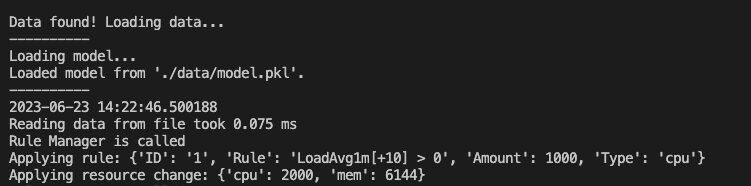
\includegraphics[width=0.8\textwidth]{chapter-4/ac-cpu.png}
    \caption{Hasil Pengujian Komponen \textit{Adaptive Control} Skenario 1: Perubahan Prosesor}
    \label{fig:ac-cpu}
\end{figure}

\begin{figure}[h]
    \centering
    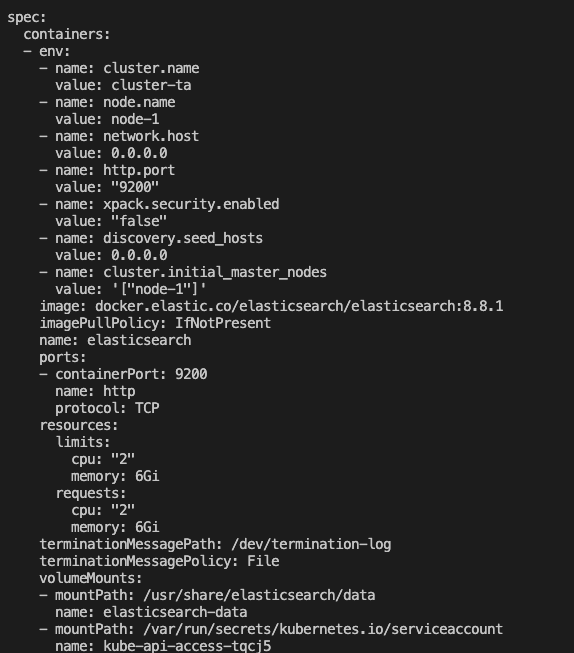
\includegraphics[width=0.8\textwidth]{chapter-4/ac-cpu-kube.png}
    \caption{Hasil Pengujian Komponen \textit{Adaptive Control} Skenario 1: Perubahan Spesifikasi Kubernetes}
    \label{fig:ac-cpu-kube}
\end{figure}

\begin{figure}[h]
    \centering
    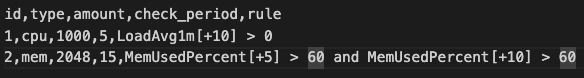
\includegraphics[width=0.8\textwidth]{chapter-4/ac-rule.png}
    \caption{File Rule untuk Pengujian Komponen \textit{Adaptive Control}}
    \label{fig:ac-rule}
\end{figure}

\begin{figure}[h]
    \centering
    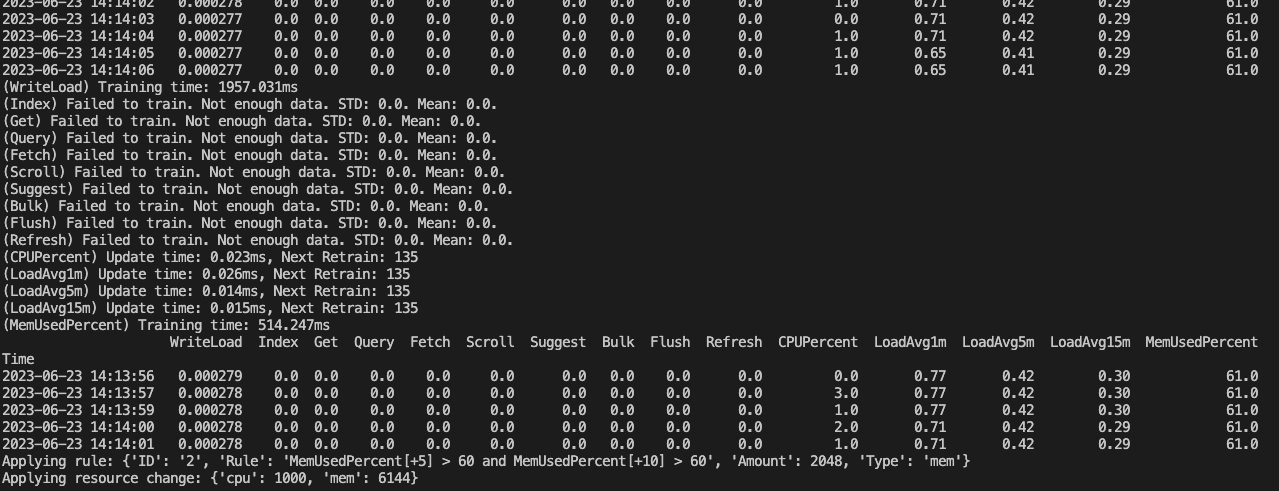
\includegraphics[width=0.8\textwidth]{chapter-4/ac-mem.png}
    \caption{Hasil Pengujian Komponen \textit{Adaptive Control} Skenario 2: Perubahan Memori}
    \label{fig:ac-mem}
\end{figure}

\begin{figure}[h]
    \centering
    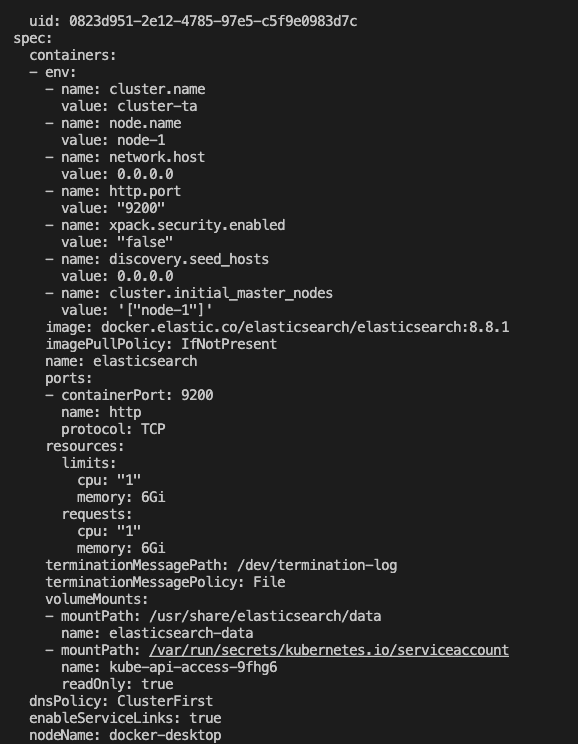
\includegraphics[width=0.8\textwidth]{chapter-4/ac-mem-kube.png}
    \caption{Hasil Pengujian Komponen \textit{Adaptive Control} Skenario 2: Perubahan Spesifikasi Kubernetes}
    \label{fig:ac-mem-kube}
\end{figure}

\begin{figure}[h]
    \centering
    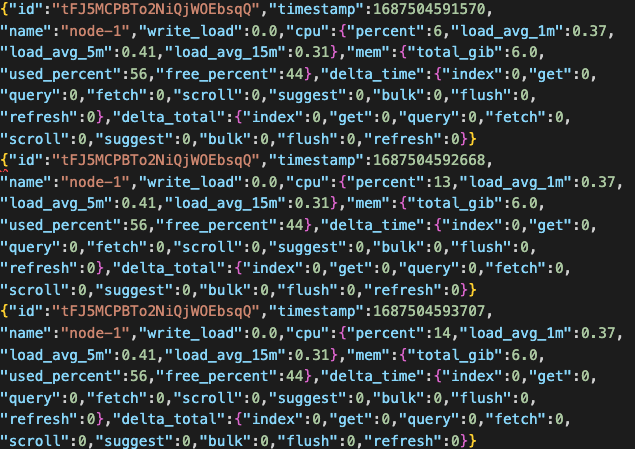
\includegraphics[width=0.8\textwidth]{chapter-4/ac-mf-turun.png}
    \caption{Hasil Pengujian Komponen \textit{Adaptive Control} Skenario 2: Perubahan Memory Used Percent pada \textit{stream file}}
    \label{fig:ac-mf-turun}
\end{figure}

Maka untuk pengujian komponen \textbf{\textit{Adaptive Control}} sudah sesuai ekspektasi dan sistem dapat berjalan dengan baik.
\chapter{Penutup}

Bab Kesimpulan dan Saran akan menjadi bagian akhir dan penutup dari penelitian tugas akhir ini. Bab ini akan membahas kesimpulan yang berisi ketercapaian tujuan penelitian tugas akhir dengan permasalahan yang diselesaikan dalam penelitian tugas akhir. Selain itu, bab ini akan membahas saran yang dapat dilakukan untuk pengembangan atau penelitian selanjutnya.

\section{Kesimpulan}
Penelitian tugas akhir ini mengimplementasikan metode baru untuk melakukan \textit{autoscaling} yang disebut sebagai sistem kontrol fleksibel. Setelah dilakukan analisis, implementasi, dan pengujian, dapat diambil kesimpulan sebagai berikut.
\begin{enumerate}
    \item Mengontrol alokasi sumber daya memori dan prosesor dapat dilakukan dengan model prediksi berbasis \textit{time series}, salah satu model yang digunakan adalah ARIMA.
    \item Dampak \textit{autoscaler} dengan kontrol fleksibel berbasis model prediksi, sistem dapat lebih baik dalam melakukan \textit{scaling} dibandingkan dengan \textit{autoscaler} sederhana yang memakai \textit{treshold} karena:

        \begin{enumerate}
            \item Dapat menghindari keputusan \textit{scaling} untuk waktu yang sangat singkat akibat \textit{spike} yang terjadi pada data metrik. Berbeda dengan sistem \textit{treshold}, yang akan langsung terpengaruh karena hanya melihat nilai metrik pada saat itu saja.
            \item Memiliki lebih banyak ruang untuk melakukan \textit{scaling} karena tidak terbatas oleh sebuah angka \textit{treshold} melainkan oleh kondisi-kondisi yang disesuaikan dengan kebutuhan pemakai.
            \item Tidak terpatok untuk melakukan \textit{scaling} dengan kelipatan minimum \textit{requirement} dari sebuah aplikasi karena replikasi \textit{pods} memaksa pengelola untuk membuat replikasi \textit{pods} (\textit{Horizontal Autoscaling}) dengan kelipatan minimum spesifikasi untuk menjalankan aplikasi tersebut.
            \item Bisa melakukan \textit{scaling} secara \textit{vertical} dengan menambah alokasi memori dan prosesor pada \textit{pods} dengan aplikasi berbasis JVM yang spesifiknya adalah \textit{Elastic Search}. \textit{Vertical Autoscaling} tidak dapat melakukan \textit{scaling} pada aplikasi berbasis JVM karena keterbatasan Kubernetes dalam melihat penggunaan memori yang sebenarnya.
            \item Dapat melakukan keputusan \textit{scaling} berdasarkan variabel-variabel yang spesifik kepada \textit{Elastic Search} seperti \textit{throughput} variabel tertentu.
        \end{enumerate}

    \item Melakukan \textit{autoscaling} tanpa melakukan \textit{restart} dapat dilakukan saat Kubernetes sudah merilis versi stabil dari 1.27 untuk melakukan \textit{In-pod resource resizing}.
\end{enumerate}

\section{Saran}
Adapun banyak kekurangan dan kelemahan yang ditemukan dalam penelitian tugas akhir ini. Berikut adalah beberapa saran yang dapat dilakukan untuk pengembangan atau penelitian selanjutnya.
\begin{enumerate}
    \item Melakukan permodelan dengan Bi-LSTM atau RNN untuk mengurangi waktu \textit{training}. Model ARIMA sangat memakan waktu saat \textit{training}.
    \item Melakukan pengembangan di bahasa lain yang lebih cepat dalam melakukan pemrosesan dibanding Python. Tentunya hal ini akan berpengaruh terhadap pembuatan kakas model statistik maupun \textit{machine learning} dikarenakan Python merupakan bahasa yang paling banyak digunakan untuk \textit{data science} dan \textit{machine learning}.
    \item Memasukkan sistem \textit{autoscaler} ke dalam \textit{cluster} Kubernetes seperti \textit{sidecar pods} agar memudahkan melakukan \textit{scaling Elastic Search} itu sendiri.
    \item Riset replikasi multi-node \textit{Elastic Search}. 
    \item Melakukan percobaan di \textit{cluster} Kubernetes dan \textit{Elastic Search} yang lebih besar dan lebih kompleks.
\end{enumerate}
%---------------------------------------------------------------%

% Daftar pustaka
\printbibliography

% Setting judul lampiran
\titlespacing*{\chapter}{0pt}{0pt}{0pt}
\titlespacing*{\section}{0pt}{0pt}{*1}

% Setting judul anak lampiran
\titleformat*{\section}{\bfseries}

\appendix

\chapter{Ilustrasi Implementasi Arsitektur VeeR EL2}
\label{appendix:veer-el2-full}

\begin{figure}[h]
	\centering
	\begin{sideways}
		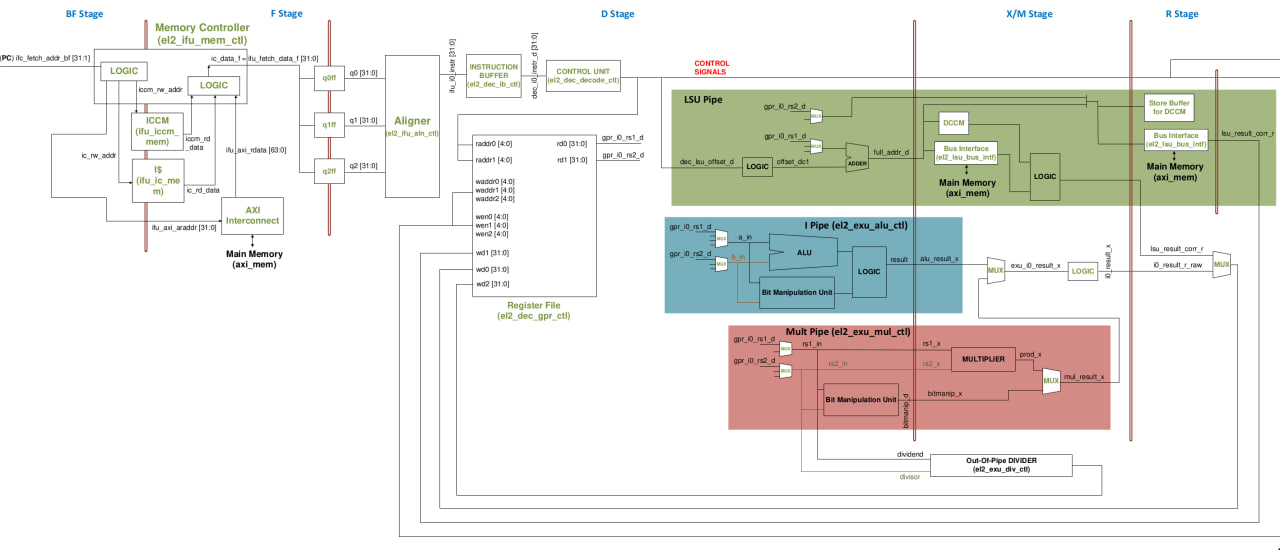
\includegraphics[width=1.3\textwidth]{chapter-3/veer-el2-full.jpg}
	\end{sideways}
	\caption{Ilustrasi Implementasi Arsiktektur VeeR EL2 \parencite{chip2024cores}}
	\label{fig:veer-el2-full}
\end{figure}

\chapter{Konfigurasi dan hasil timing diagram dari Verilator}
\label{appendix:verilator}

Terdapat dua unit pengujian yang dilakukan untuk mengetahui akurasi yang dimiliki oleh akselerator: q.max dan q.update. Instruksi lain, digunakan dan diuji sekaligus untuk menguji kedua instruksi tersebut.

Pertama, pengujian q.max, dilakukan dengan membuat sebuah program pada bahasa C pada gambar \ref{fig:verilator-qmax}.

\begin{figure}[H]
	\centering
	\begin{lstlisting}[language=C,escapechar=|,numbers=left]
int main() {
  setAMax(4);
  storeQValue(10.2, 0);
  storeQValue(6.2, 1);
  storeQValue(3.2, 2);
  storeQValue(12.0, 3);
  getMax(0);
}
\end{lstlisting}
	\caption{Program bahasa C untuk pengujian q.max}
	\label{fig:verilator-qmax}
\end{figure}

Hasil dari program diatas, seharusnya menghasilkan indeks 3 sebagai jawaban dari fungsi getMax yang merupakan \ac{BSP} dari q.max. Berikut merupakan hasil sintesis \textit{timing diagram} untuk program \ref{fig:verilator-qmax}.

\begin{figure}[h]
	\centering
	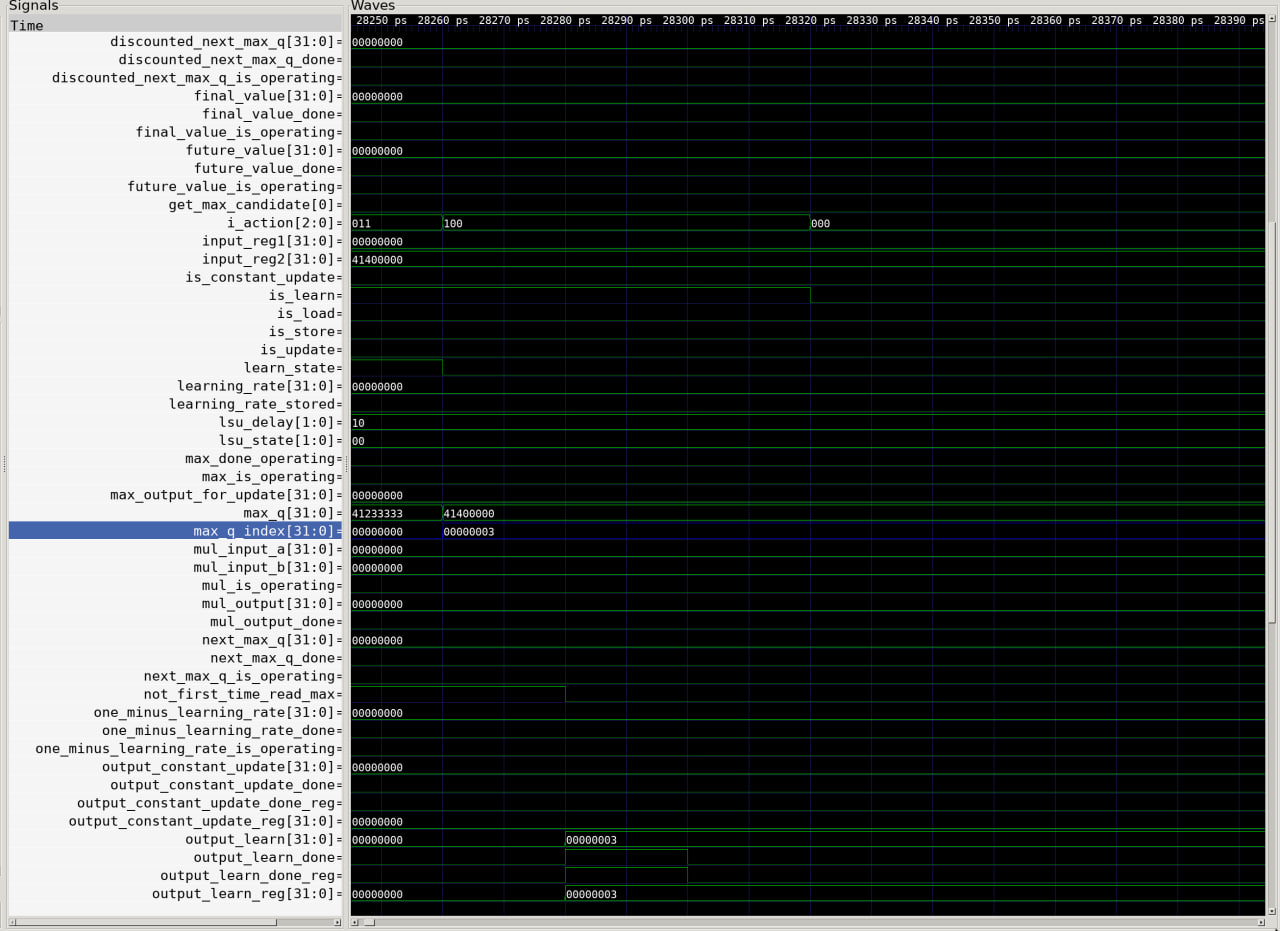
\includegraphics[width=1\textwidth]{appendix/gtkwave-qmax.jpg}
	\caption{Hasil \textit{timing diagram} program q.max}
	\label{fig:gtkwave-qmax}
\end{figure}

Dapat diperhatikan pada gambar \ref{fig:gtkwave-qmax}, bahwa nilai keluaran \textit{max\_q\_index} yang merupakan representasi $a_{max}$ itu bernilai 3. Maka, hasil dari akselerator sudah sesuai untuk instruksi q.max.

Selanjutnya, untuk instruksi q.update, berikut merupakan program yang digunakan untuk menguji akurasi akselerator.


\begin{figure}[H]
	\centering
	\begin{lstlisting}[language=C,escapechar=|,numbers=left]
int main() {
  setAMax(4);
  setConstant(CONSTANT_TYPE_LEARNING_RATE, 0.4);
  setConstant(CONSTANT_TYPE_DISCOUNT_FACTOR, 0.28);
  storeQValue(10.2, 0);
  storeQValue(6.2, 1);
  storeQValue(3.2, 6);
  storeQValue(12.0, 12);
  setNextState(1);
  qUpdate(0, 2.5);
}
\end{lstlisting}
	\caption{Program bahasa C untuk pengujian q.update}
	\label{fig:verilator-qupdate}
\end{figure}

Bila menggunakan persamaan \ref{eq:q-learning}, maka didapat nilai hasil dari gambar \ref{fig:verilator-qupdate} adalah 8.26. Nilai tersebut, bila diubah ke heksadesimal maka akan bernilai 0x410432cb. Program \ref{fig:verilator-qupdate} kemudian dicoba dan didapatkan hasil pada gambar \ref{fig:gtkwave-qupdate}.

\begin{figure}[h]
	\centering
	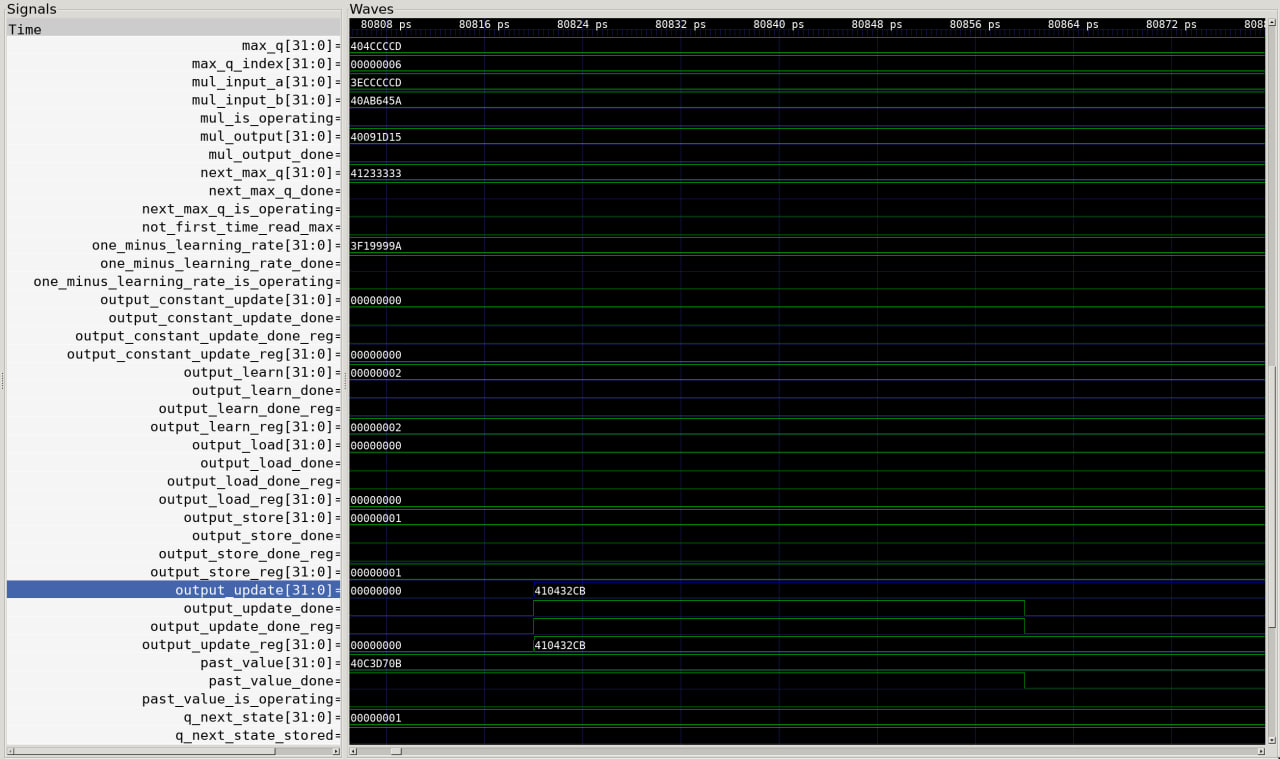
\includegraphics[width=1\textwidth]{appendix/gtkwave-qupdate.jpg}
	\caption{Hasil \textit{timing diagram} program q.update}
	\label{fig:gtkwave-qupdate}
\end{figure}

Dapat dilihat, pada gambar \ref{fig:gtkwave-qupdate}, didapat hasil pada \textit{register} \textit{output update} yang bernilai 0x410432cb. Sehingga, akselerator sudah terimplementasikan secara akurat.



\end{document}
